%!TEX TS-program = xelatex
%!TEX encoding = UTF-8 Unicode
\documentclass{icisfinal}
\usepackage{graphicx}
\usepackage{subcaption}
\graphicspath{ {imagenes/} }
\title{Music Information Retrieval: Similitud de géneros musicales}
\researchtype{Clustering}
\shorttitle{MIR: Géneros musicales}
\track{Clustering música}

\usepackage[hidelinks]{hyperref}
\addbibresource{references.bib}

\usepackage{tabularx}  % To have the table fill out the page
\usepackage{multirow}
\usepackage{setspace} % To doublespacing
\usepackage{caption}
\usepackage{float}

\captionsetup{width=0.8\linewidth}

\begin{document}
\author{Daniel Caicedo, Ignacio Chiapella, Miguel Guerrero, Juan Knebel}
\maketitle

\begin{table}[h!]
  \centering
  \LARGE
  \begin{tabularx}{\textwidth}{@{}*2{>{\centering\arraybackslash}X}@{}}
    \textbf{Daniel Caicedo}        & \textbf{Ignacio Chiapella} \\
    UAH & FCEyN   \\
    djcc710@gmail.com & ignacio.chiapella@gmail.com \\
    \\
    \textbf{Miguel Guerrero}        & \textbf{Juan Knebel} \\
    CUFM & FCEyN   \\
    miguelgh72@gmail.com & juanknebel@gmail.com \\
    \\
  \end{tabularx}
\end{table}

\begin{abstract}
  Escribir resumen del articulo

  \emph{\textbf{Keywords:} Cluster, DataMining, Música, KMeans, KMedoids, DBSCAN, Hierarchical, Silhouette, PCA, Distancias, MIR}
\end{abstract}

\section{Introducción}
\textit{La recuperación de información musical}, \textbf{Music Information Retrieval} en inglés o simplemente \textbf{MIR} de ahora en adelante, es la ciencia interdisciplinaria encargada de recuperar información de la música. Decimos que es interdisciplinaria ya que principalmente los especiales en musicología, en procesamiento de señales o en aprendizaje automático son los que más implicados en el tema están.

Actualmente \textbf{MIR} es un área de estudio nuevo pero en crecimiento y muchos de sus estudios y resultados están siendo utilizados en muchas aplicaciones comerciales desde sistemas de recomendación, búsqueda de contenido, interfaces de usuarios para navegar por grandes colecciones de música, detección de instrumentos, categorización automática y hasta generación de música.

Si bien el estudio de la música y la importancia que tuvo y sigue teniendo a lo largo de la historia no tiene discusión, en los últimos años el estudio de la técnica cobro mayor notoriedad. Las causas de lo anteriormente mencionado son, (i) el avance tecnológico que posibilitó a todos tener acceso a prácticamente cualquier pista de audio gracias a aplicaciones como \textit{Napster}, \textit{Grooveshark} y recientemente \textit{Spotify}, (ii) el incremento del poder de computo para aplicar las técnicas de estudio de la música, solo por nombrar dos de ellas.

En este trabajo se realizará un estudio sobre los atributos de más de 2000 canciones, los cuales fueron obtenidas de la interfaz que ofrece Spotify. En la primer sección se comentarán los atributos.

El trabajo consistirá en aplicar diferentes técnicas de \textbf{Clustering} sobre los conjuntos de datos previamente mencionados. El objetivo será agrupar diferentes canciones según su similitud en términos del género musical al que pertenecen.

Las técnicas que se utilizarán serán el clásico método \textit{KMeans}, seguido por el también clásico pero más robusto al ruido \textbf{PAM} o \textbf{KMedoids}, también utilizaremos una implemetanción jerárquica o \textbf{Hierarchical}. Por último mencionaremos una experiencia fallida con el método \textbf{DBSCAN}, anticipando que en principio y para este conjunto de datos las pistas de audio no tienen un agrupamiento por densidad.

\section{Trabajo previo}
Antes de comenzar con el trabajo actual, es necesario describir el conjunto de datos con el cual se realizaron las experimentaciones. El primer archivo llamado "audio\_features" contiene los atributos llamados de alto nivel de los cuales solo tuvimos en cuenta los siguientes: acousticness, danceability, energy, instrumentalness, liveness, loudness, speechiness, tempo y valence. El resto fueron dejados lado ya que no aportaban ningún valor para el agrupamiento de las canciones. Por ejemplo: analysis\_url, track\_href, type y uri fueron inmediatamente descartadas ya que es información vinculada a la extracción de datos. El resto: duration\_ms, key, mode y time\_signature no ayudan en nada a discriminar grupos de canciones, como puede verse en el siguiente gráfico.

\begin{figure}[H]
    \centering
    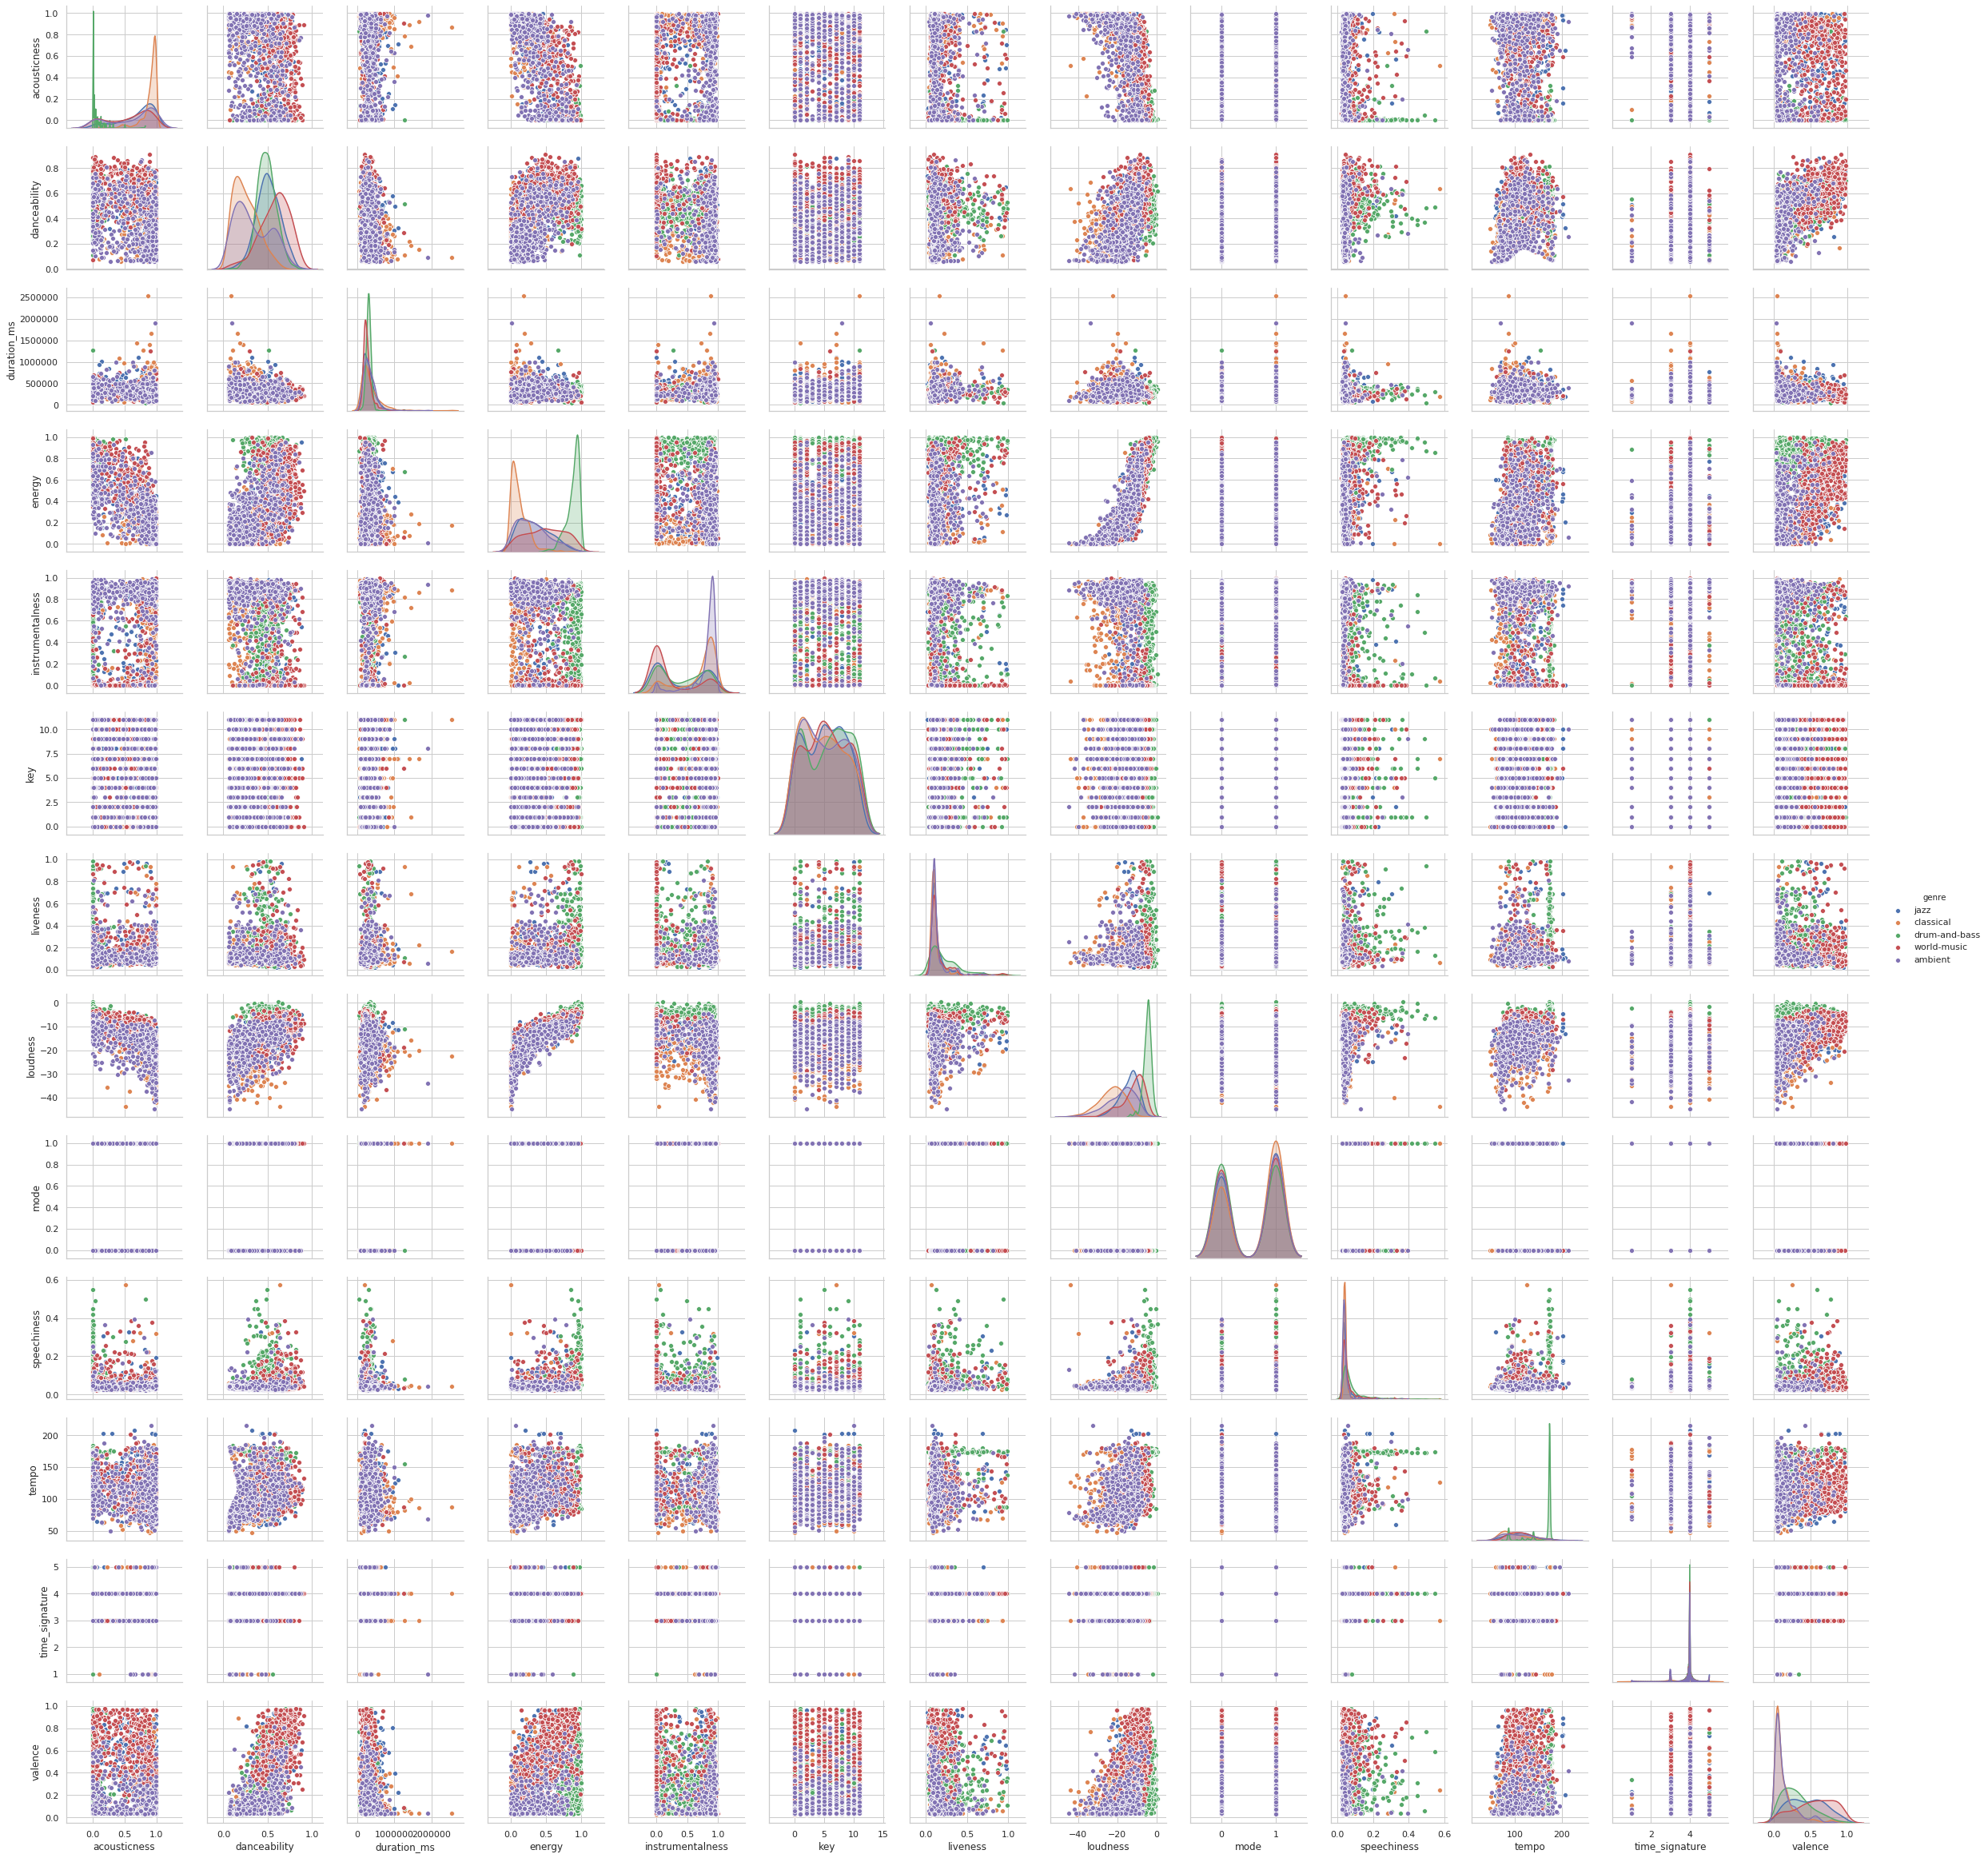
\includegraphics[width = 4in]{img/scatter-af-complete.png}
    \caption{Scatter plot de los atributos de alto nivel.}
    \label{fig:scatter-af}
\end{figure}

El segundo conjunto de archivos llamados "audio\_analysis" contienen 12 atributos de bajo nivel, uno para cada una de las notas musicales. Se cuenta con un archivo por pista tanto para el timbre como para el pitch separados en ventanas de tiempo. Para no trabajar con series de tiempo y porque las pistas tiene duraciones distintas, se resumieron estos atributos en 2 medidas distintas tanto para los pitches como para los timbres. Las medidas elegidas fueron: para cada atributo de cada canción se calculo la media total y el desvío estándar. Entonces por cada uno de los temas musicales obtuvimos 2 valores resúmenes para cada uno de los 12 atributos. Para el trabajo posterior no se descartó ningún atributo ya que todos son importantes para el agrupamiento.

\begin{figure}[H]
    \begin{subfigure}{.4\textwidth}
        \centering
        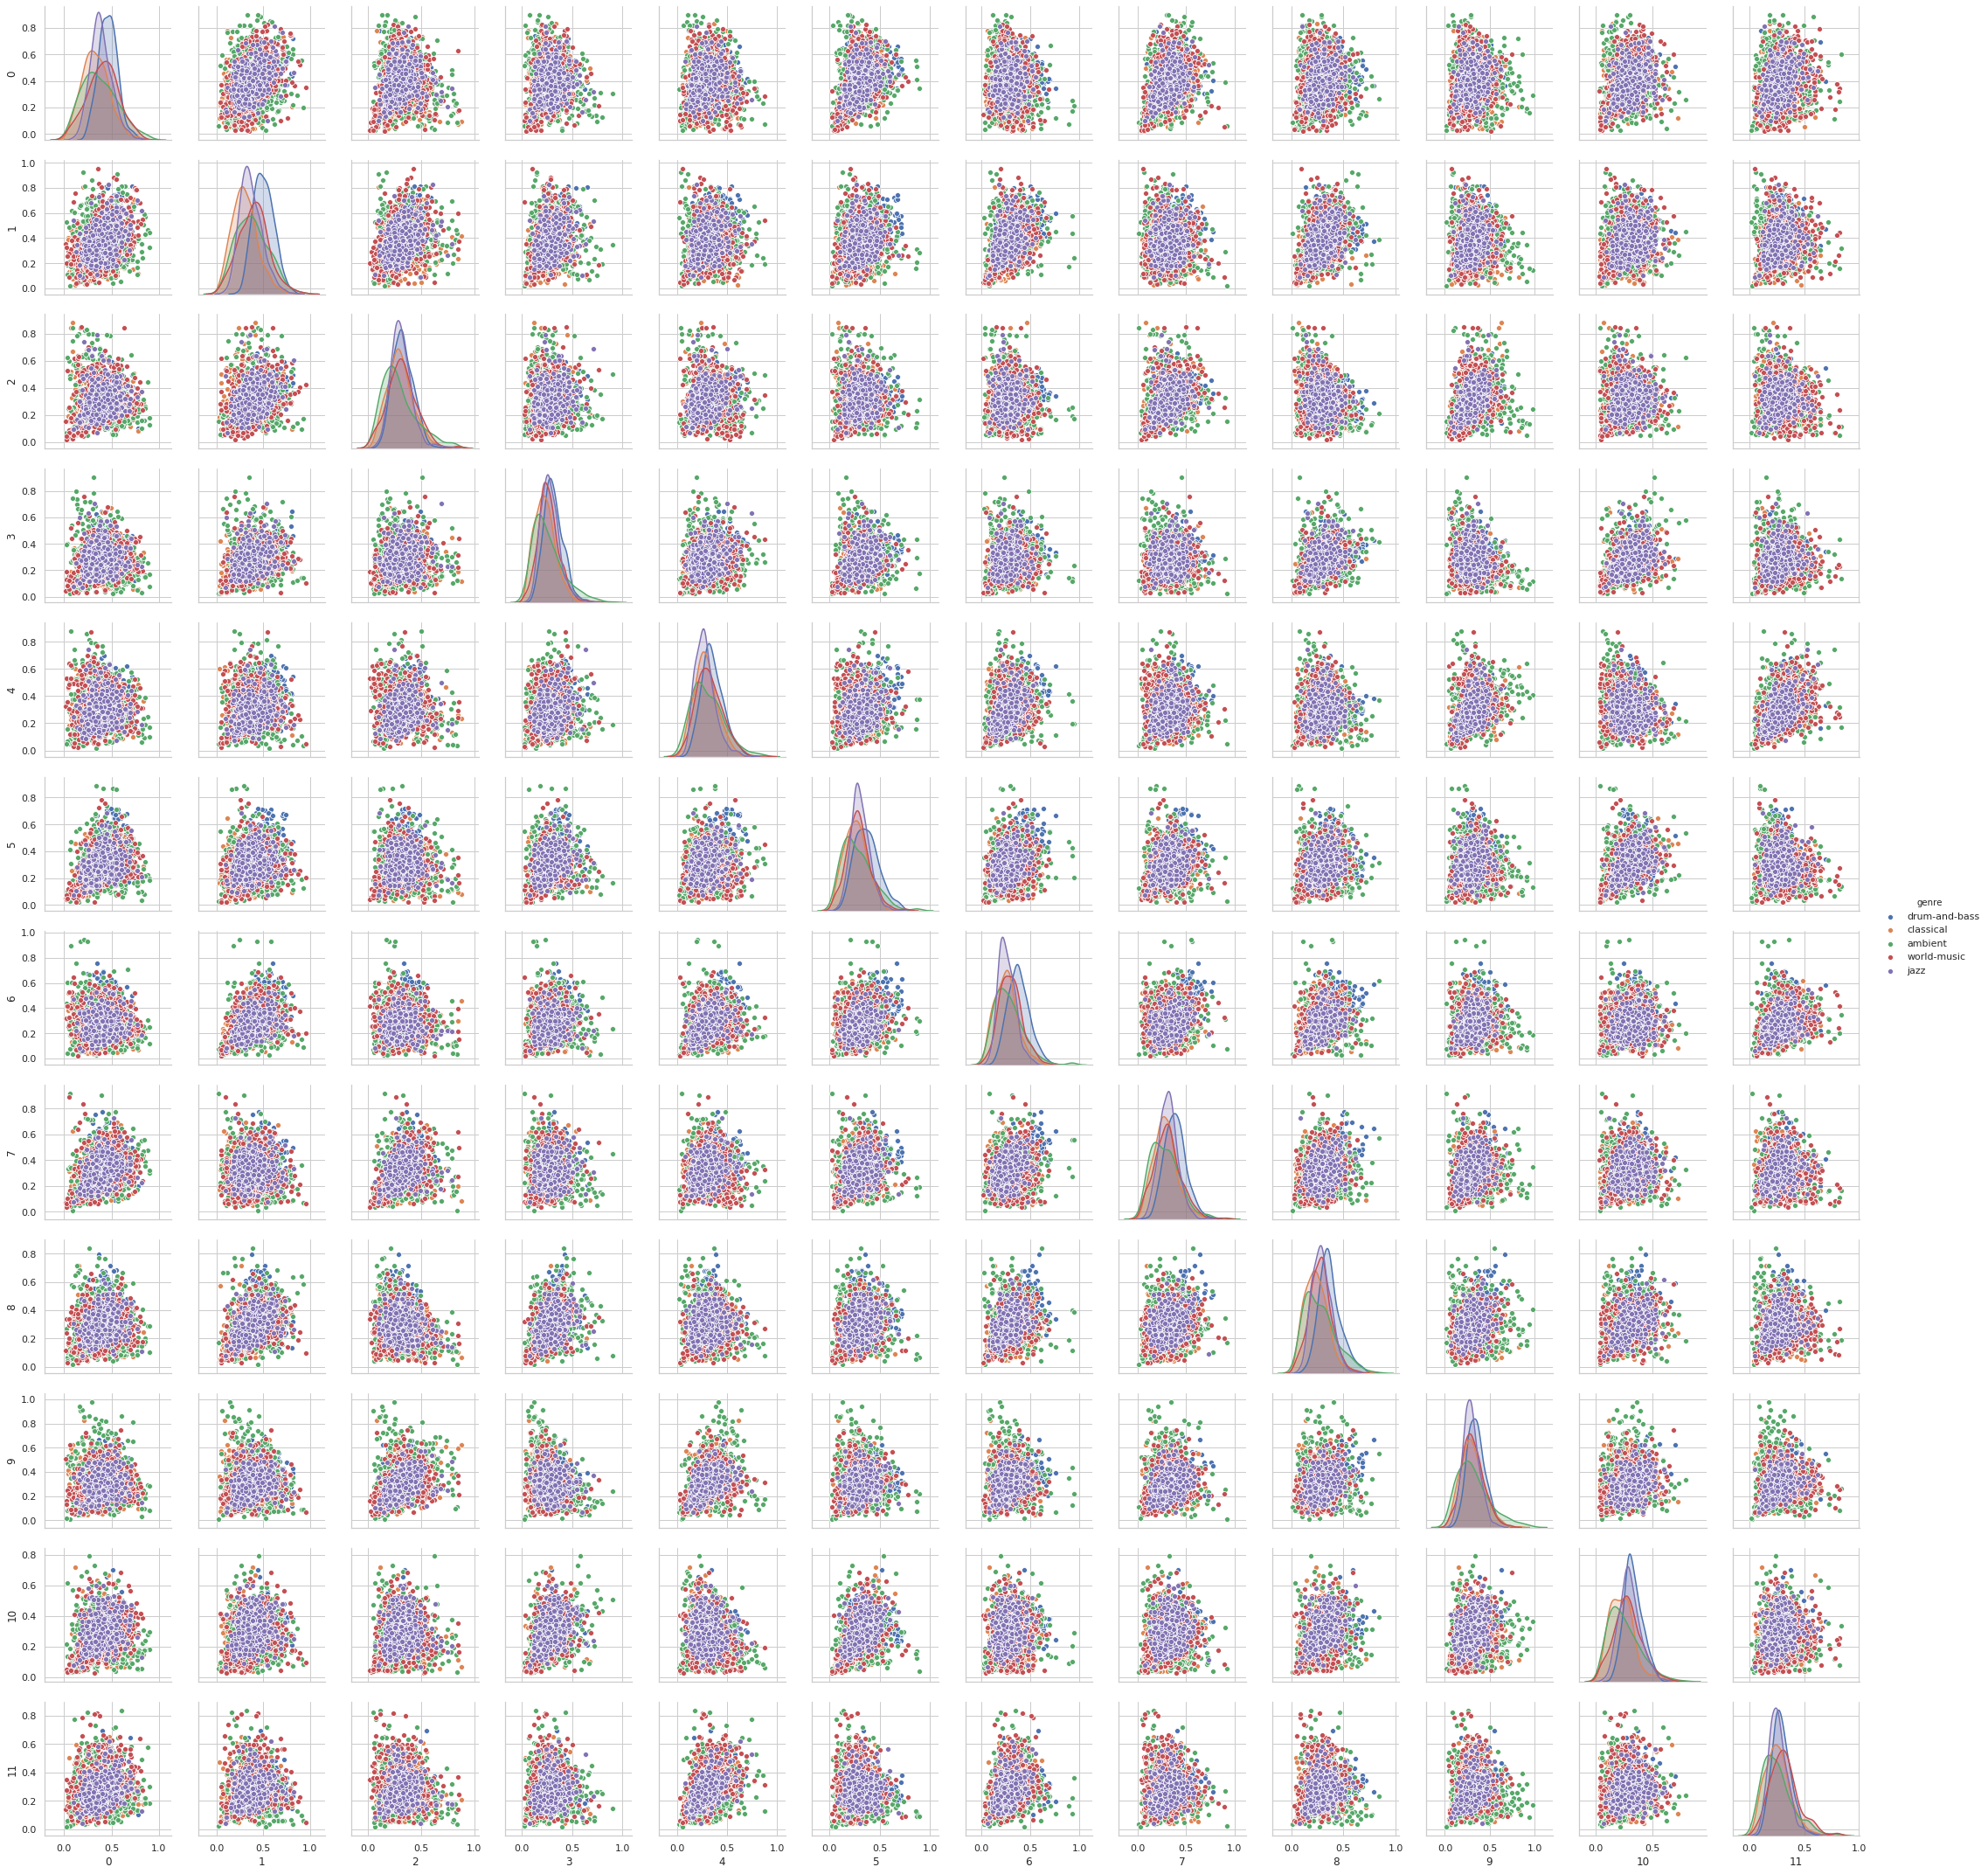
\includegraphics[width = 2in]{img/scatter-aa-pitches-avg.png}
    \end{subfigure}
    \begin{subfigure}{.4\textwidth}
        \centering
        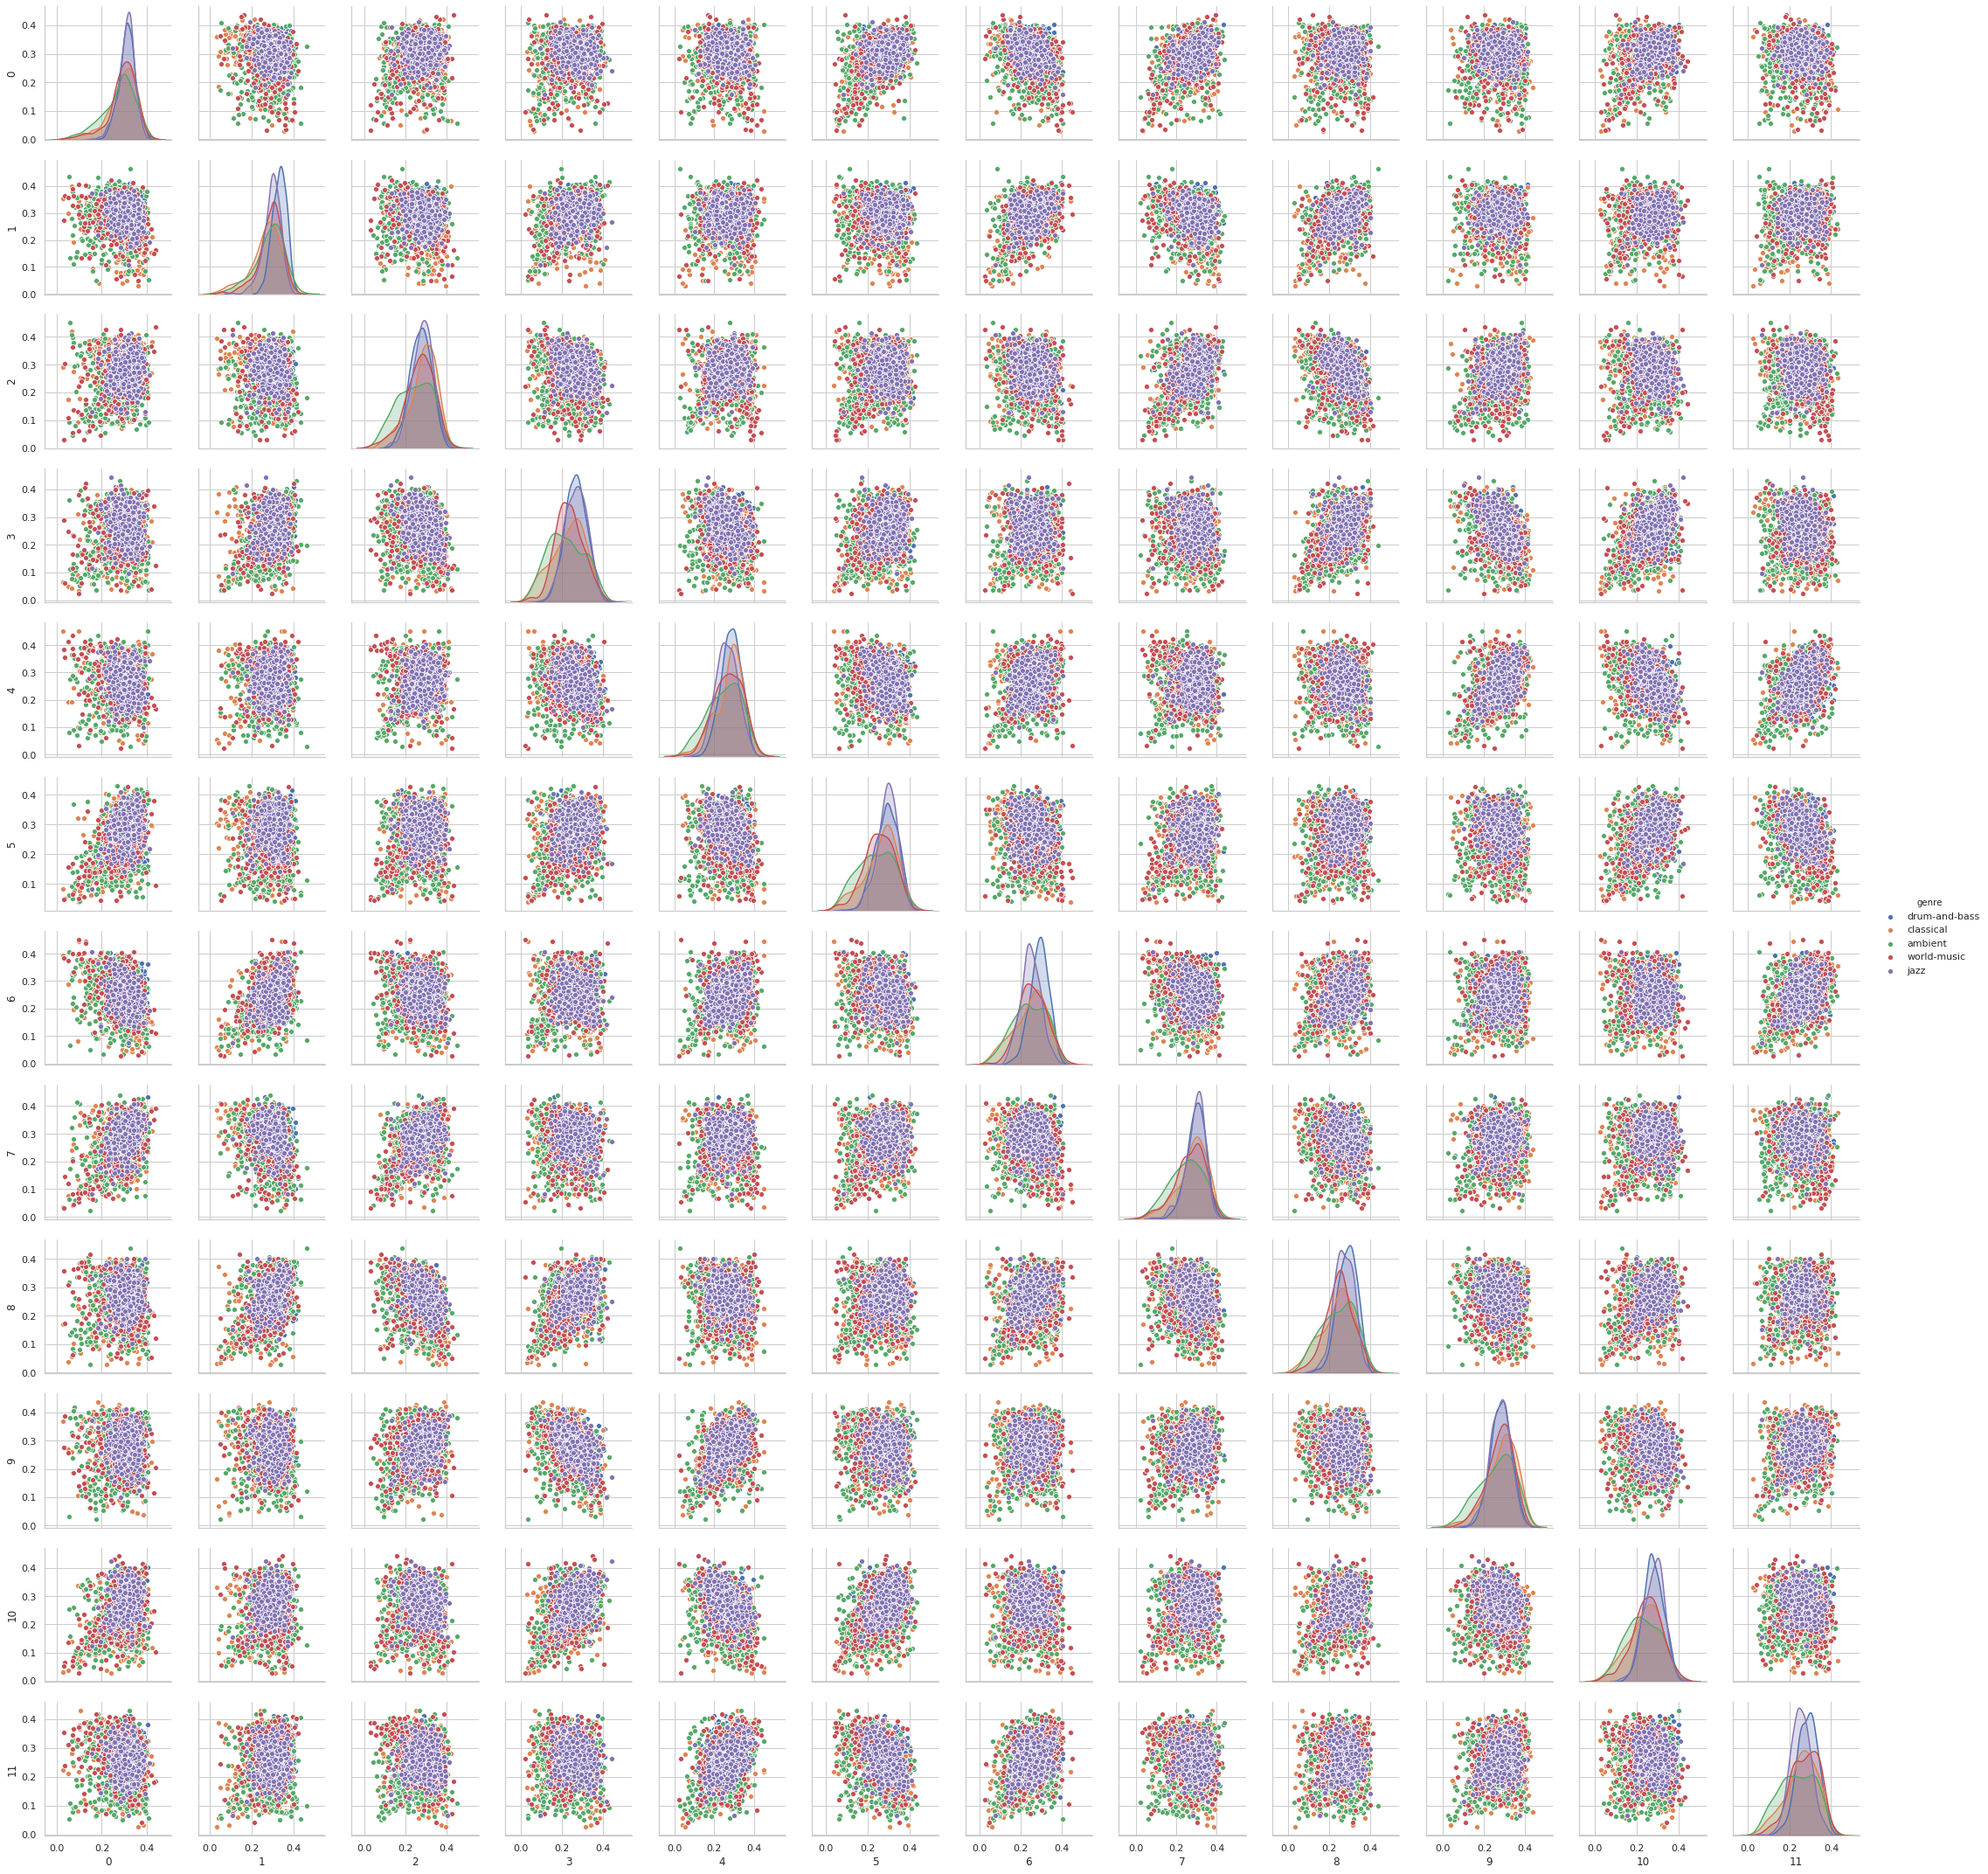
\includegraphics[width = 2in]{img/scatter-aa-pitches-std.png}
    \end{subfigure}
    \caption{Scatter plot de los atributos sobre el pitch.}
    \label{fig:scatter-aa-pitches}
\end{figure}

\begin{figure}[h]
    \begin{subfigure}{.4\textwidth}
        \centering
        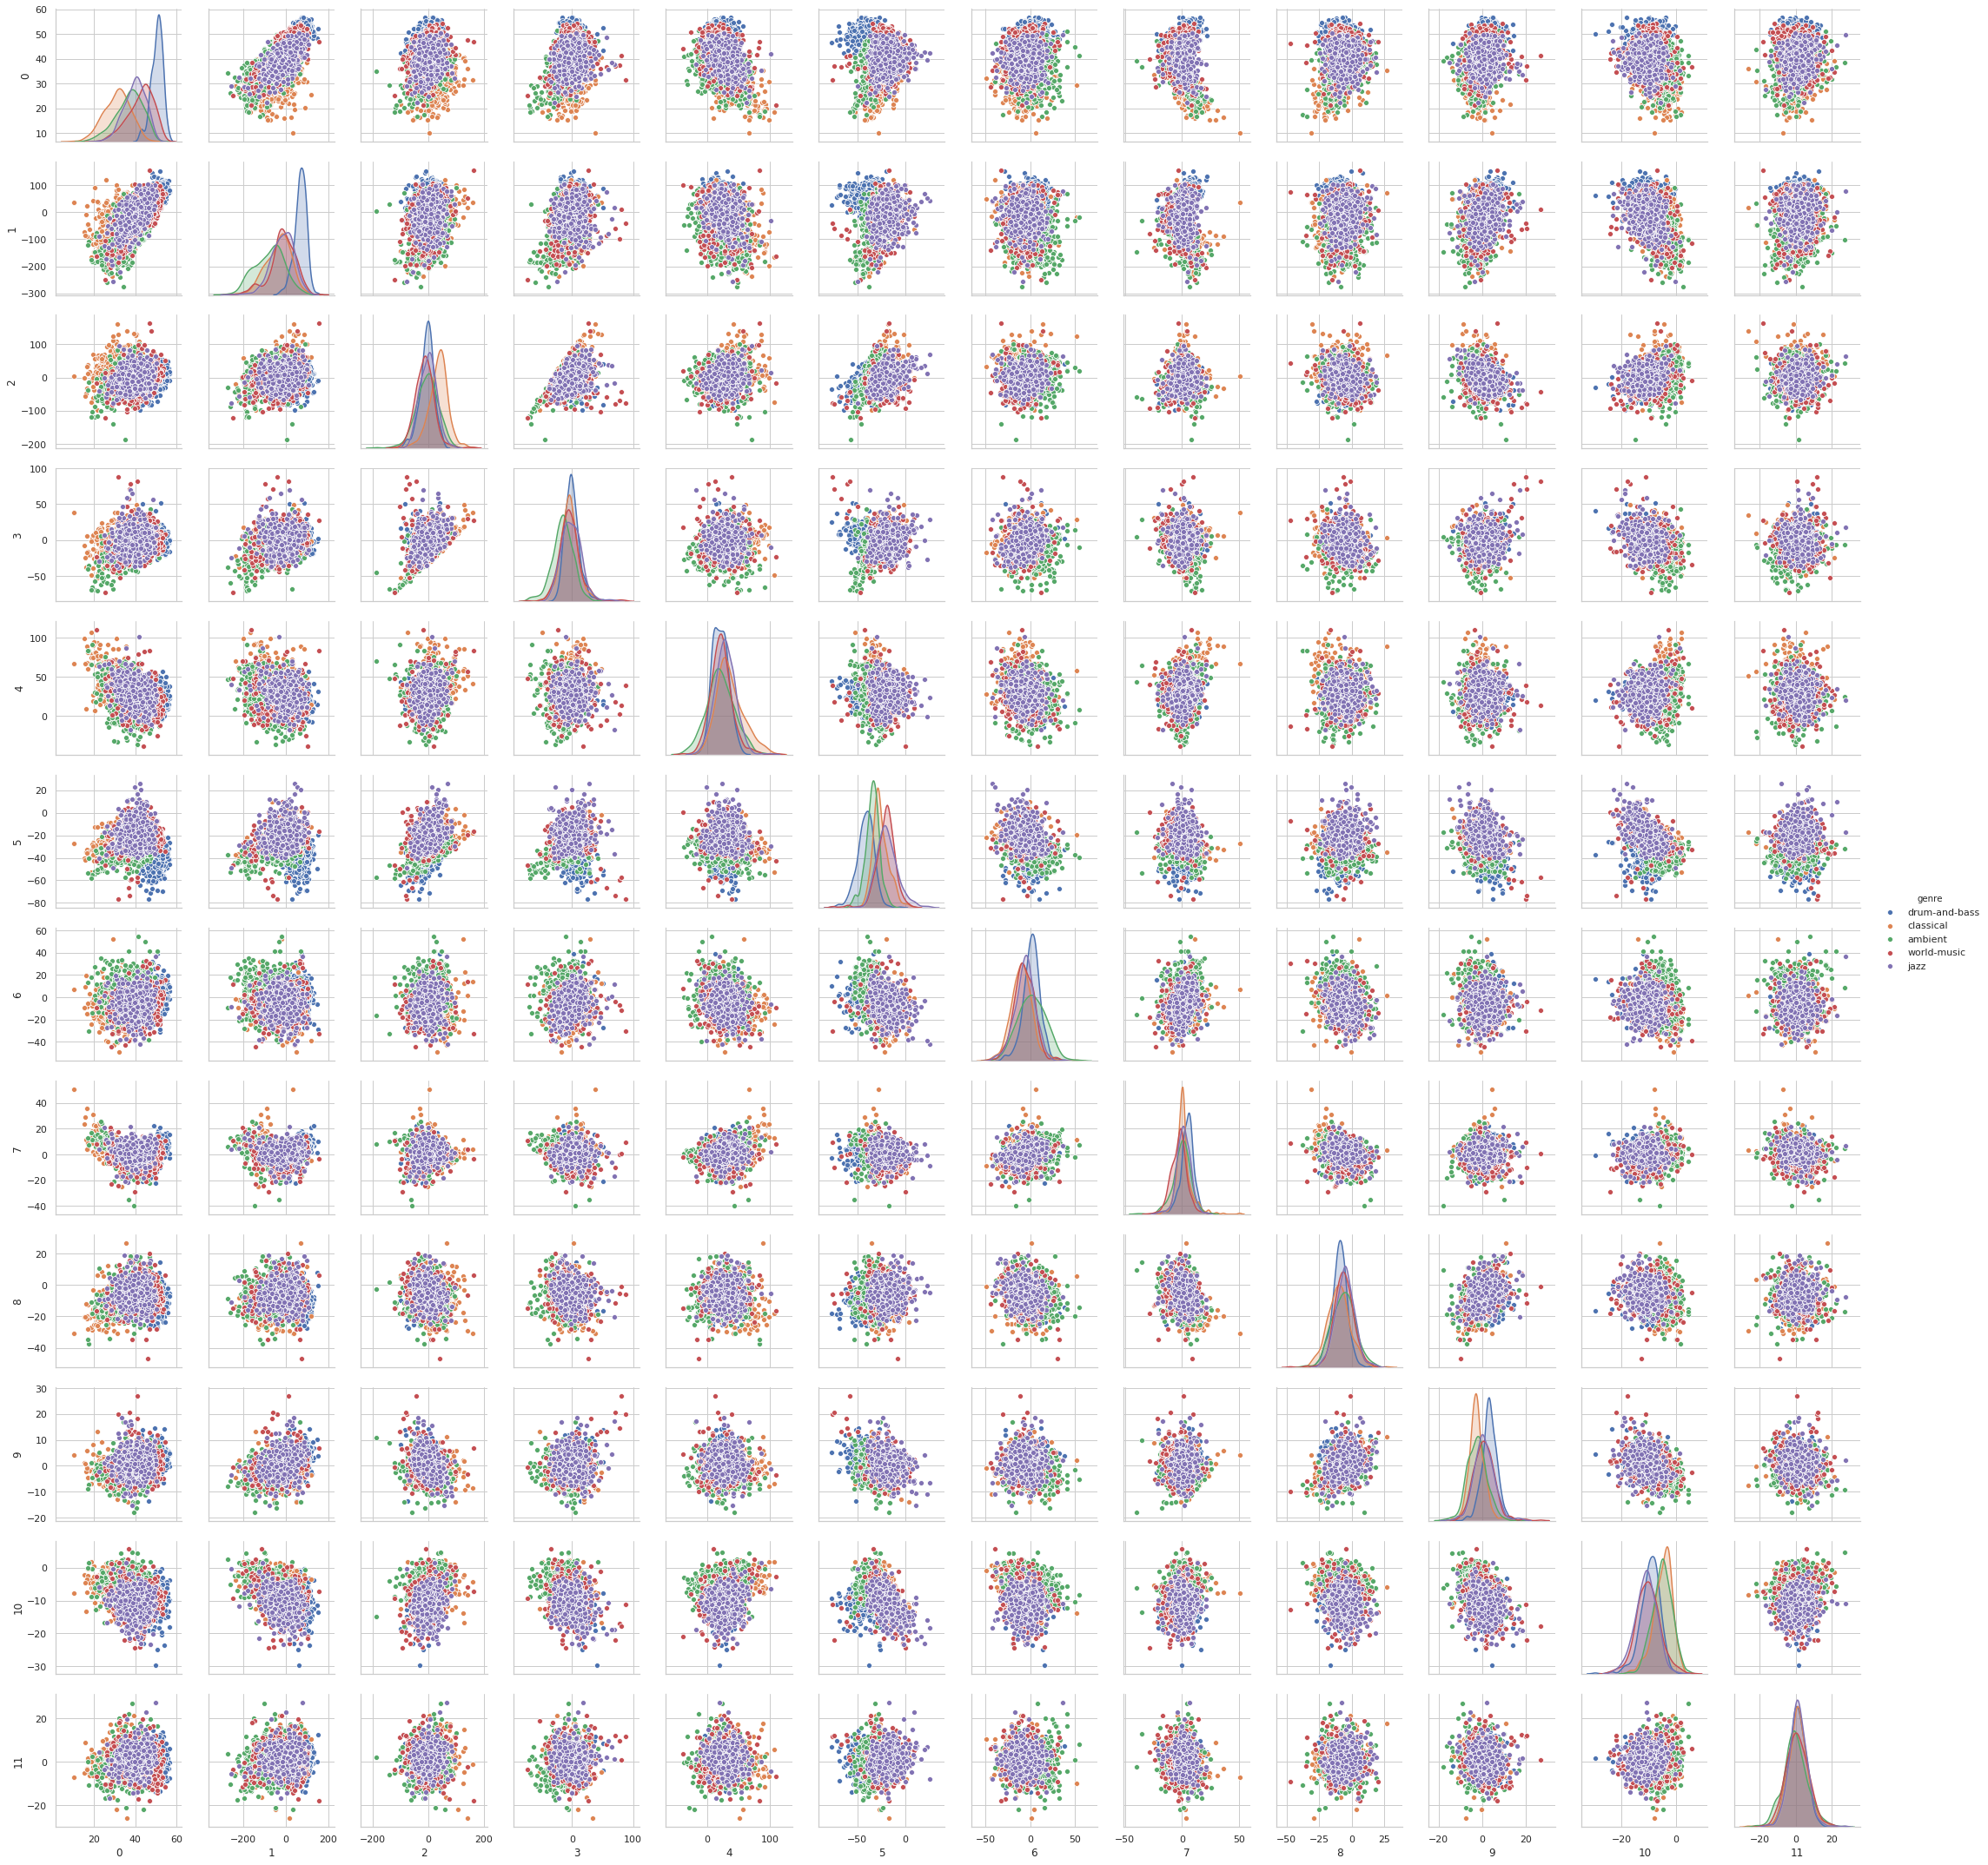
\includegraphics[width = 2in]{img/scatter-aa-timbres-avg.png}
    \end{subfigure}
    \begin{subfigure}{.4\textwidth}
        \centering
        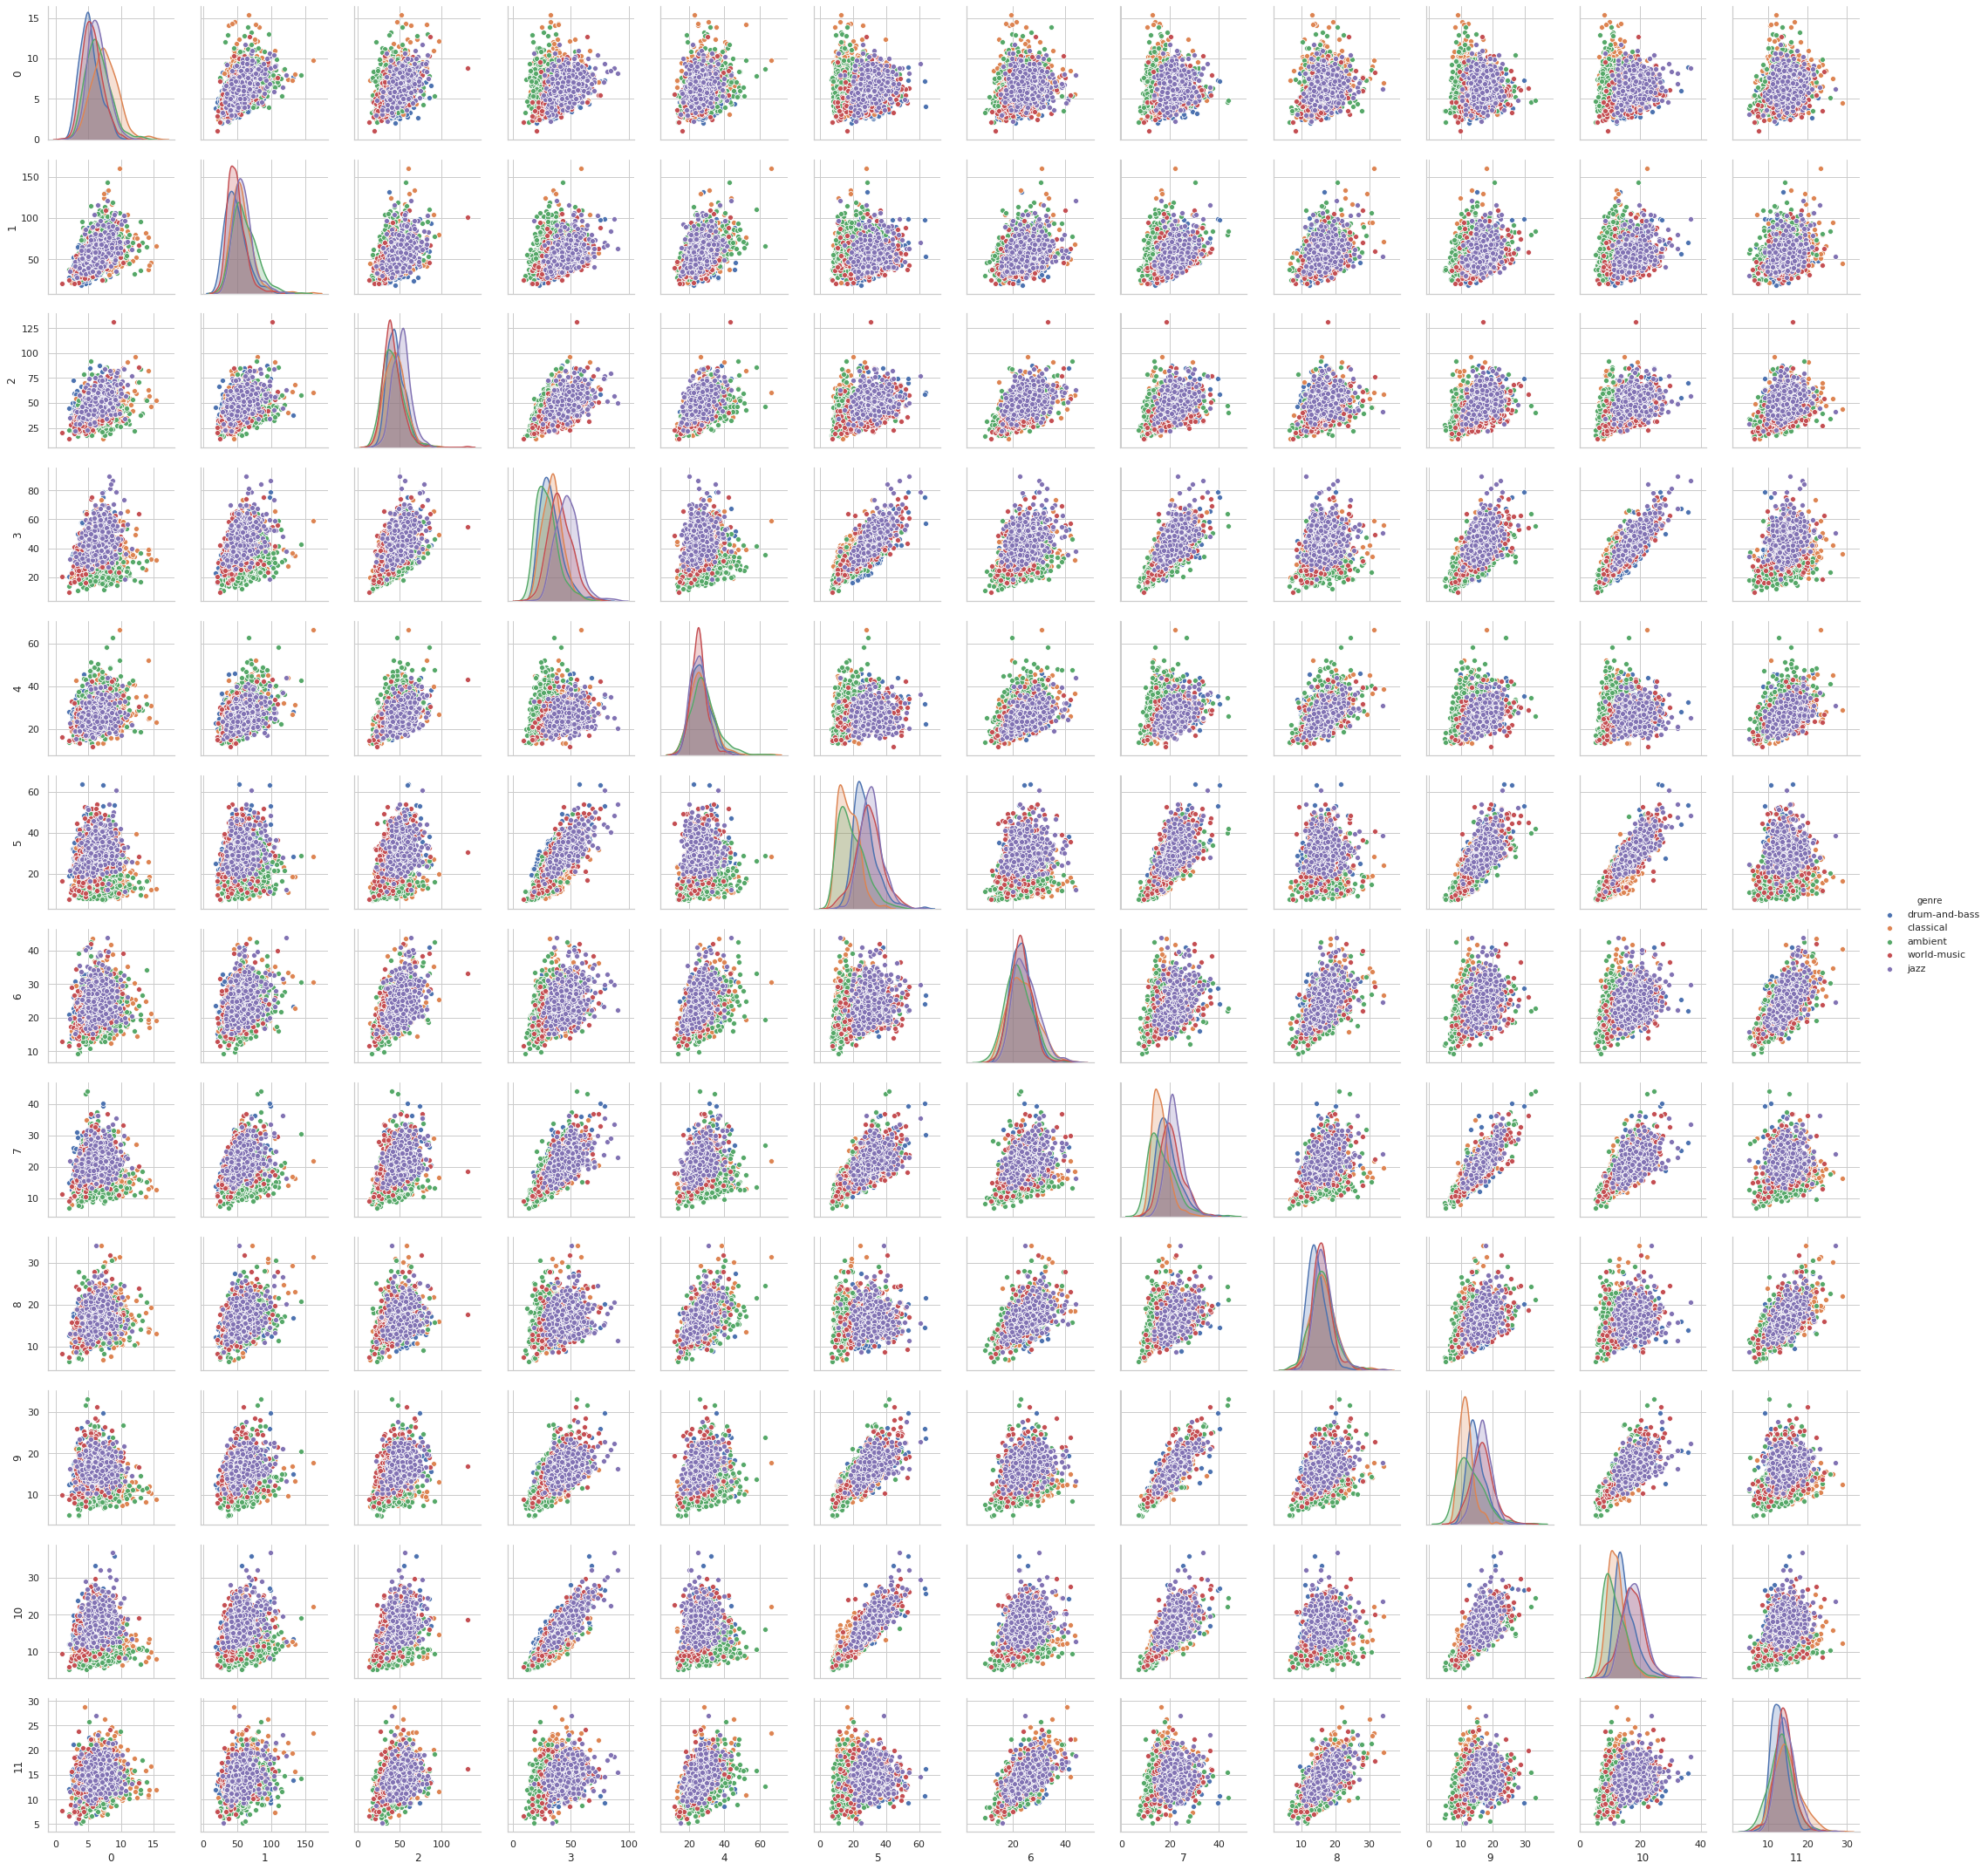
\includegraphics[width = 2in]{img/scatter-aa-timbres-std.png}
    \end{subfigure}
    \caption{Scatter plot de los atributos sobre el timbre.}
    \label{fig:scatter-aa-timbres}
\end{figure}

Todas las canciones de este conjunto de datos pertenecen a solo 5 géneros musicales: ambient, classical, drum and bass, jazz y world music.

\newpage
\section{Experiencia KMeans}
Se utilizó el algoritmo \textbf{KMeans} de la librería \textbf{Scikit Learn} \autocite{scikit-learn} con la utilización de sus parámetros por defecto \autocite{sklearn\_api}. Al tratarse de un método sin supervisión necesitamos indicarle la cantidad de clusters en las cuales se quiere que estén agrupadas las observaciones.

Para medir que tan "bien" resulta la agrupación vamos a utilizar diferentes medidas. La primera para identificar cual será la cantidad de clusters será utilizar la suma de los errores cuadrados medios, o \textbf{SSE} por sus siglas en inglés. También nos apoyaremos en la medida de \textbf{silhouette} para observar que cantidad de clusters obtuvo el mejor valor y también para validar la consistencia de los clusters obtenidos. Como métrica adicional para validar la consistencia de los grupos generados \textbf{Rand index}.

Comenzaremos con generar entre 2 a 6 clusters para los atributos de alto nivel, luego elegida la cantidad de clusters vamos a proceder a agrupar las mismas canciones pero utilizando los datos de bajo nivel, recordar que usaremos las 4 medidas que resumen la información y obtuvimos en el trabajo previo. Con estos nuevos resultados se elegirá cual fue la medida que obtuvo mejores métricas y procederemos a concatenar los valores de alto nivel con esta última. Con este nuevo conjunto de generado vamos a recrear el experimento de generar de 2 a 6 clusters y observar si los resultados se repiten o no.
\subsection{Resultados}
\subsubsection{Atributos de alto nivel}
Vamos a comenzar analizando cual sería la mejor cantidad de clusters para los atributos de alto nivel.

\begin{figure}[H]
    \begin{subfigure}{.4\textwidth}
        \centering
        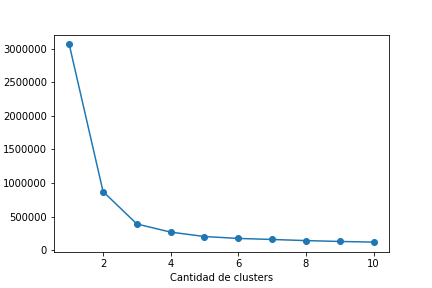
\includegraphics[width = 2in]{img/kmeans/elbow.png}
        \caption{Método elbow}
    \end{subfigure}
    \begin{subfigure}{.4\textwidth}
        \centering
        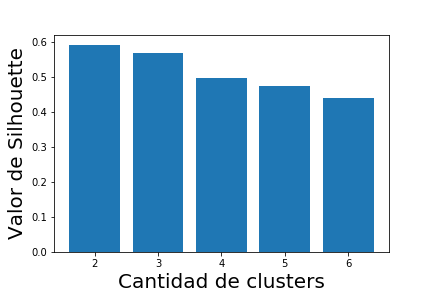
\includegraphics[width = 2in]{img/kmeans/silhouette-features.png}
        \caption{Silhouette score}
    \end{subfigure}
    \caption{Cantidad de clusters óptima}
    \label{fig:elbow-silhouette}
\end{figure}

Si solo tuviésemos en cuenta el método elbow podríamos elegir 4 clusters como el óptimo para realizar el agrupamiento pero, al observar los valores que se obtienen con el método del silhouette, se decidió que el número de clusters sea 3.

\begin{table}[H]
    \centering
    \begin{tabular}{|c|c|}
        \hline
        Cantidad de clusters & Indice de Rand \\
        \hline
        2 & 0.098 \\
        3 & 0.122 \\
        4 & 0.141 \\
        5 & 0.146 \\
        6 & 0.152 \\
        \hline
    \end{tabular}
    \caption{Rand index}
    \label{tab:rand-kmeans-af}
\end{table}

Para reforzar la elección de 3 como cantidad de clusters se puede apreciar que quitando un agrupamiento de 2 clusters, el resto de valores fue cambiando pero no tan abruptamente.

A continuación se muestra la tabla que se obtiene de evaluar los el método con 3 clusters en que grupo clasificó a cada pista musical.

\begin{table}[H]
    \centering
    \begin{tabular}{|c|c|c|c|}
        \hline
        & \multicolumn{3}{ c| }{Clusters} \\
        \hline
        Género & 0 & 1 & 2 \\
        \hline
        ambient & 224 & 58 & 178 \\
        classical & 253 & 32 & 120 \\
        drum-and-bass & 39 & 359 & 53 \\
        jazz & 159 & 56 & 212 \\
        world-music & 182 & 62 & 219 \\  
        \hline
    \end{tabular}
    \caption{Géneros musicales y grupos}
    \label{tab:cross-kmeans-af-3}
\end{table}

El género \textbf{drum-and-bass} es el que mejor concentración presenta en el cluster número 1, este mismo también presenta muy pocas observaciones del resto de los géneros musicales. Por último los clusters 0 y 2 contienen de forma balanceanda el resto de los géneros. Se podría sospechar que al menos para los atributos de alto nivel el género \textbf{drum-and-bass} se encuentra mas separado del resto de los estilos musicales. A modo de comparación vamos a incluir una tabla similar a ~\ref{tab:cross-kmeans-af-3} pero con 5 clusters. Y si observará el mismo comportamiento solo que esta vez el cluster 2 es quien concentra al estilo \textbf{drum-and-bass}.

\begin{table}[H]
    \centering
    \begin{tabular}{|c|c|c|c|c|c|}
        \hline
        & \multicolumn{5}{ c| }{Clusters} \\
        \hline
        Género & 0 & 1 & 2 & 3 & 4 \\
        \hline
        ambient & 90 & 124 & 43 & 106 & 97 \\
        classical & 52 & 157 & 28 & 77 & 91 \\
        drum-and-bass & 41 & 1 & 357 & 14 & 38 \\
        jazz & 86 & 57 & 48 & 136 & 100 \\
        world-music & 94 & 29 & 45 & 145 & 150 \\
        \hline
    \end{tabular}
    \caption{Géneros musicales y grupos}
    \label{tab:cross-kmeans-af-4}
\end{table}

\subsubsection{Atributos de bajo nivel}
En este caso ya decidimos que la cantidad de clusters serán 3, entonces para comenzar a evaluar que conjunto de medidas resúmenes (media y desvío estándar de timbres y pitches) es la más efectiva calculamos el valor de silhouette para cada uno de ellos.

\begin{figure}[H]
    \centering
    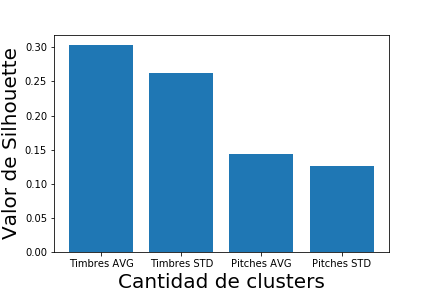
\includegraphics[width = 4in]{img/kmeans/silhouette-analysis.png}
    \caption{Silhouette}
    \label{fig:silhouette-aa-3-all}
\end{figure}

El pitch obtuvo valores muy bajos en comparación al timbre y de éste último vamos a explorar usando la medida de la media que obtuvo mejores valores. Adjuntamos la tabla con los valores del índice de Rand que refuerzan la elección ya que se obtuvieron valores muy superiores que con el resto de las medidas.

\begin{table}[H]
    \centering
    \begin{tabular}{|c|c|}
        \hline
        Conjunto de medidas resumenes & Indice de Rand \\
        \hline
        timbre y su media & 0.151 \\
        timbre y su desvío estándar & 0.084 \\
        pitch y su media & 0.096 \\
        pitch y su desvío estándar & 0.030 \\
        \hline
    \end{tabular}
    \caption{Rand index}
    \label{tab:rand-kmeans-aa-3-all}
\end{table}

Ahora analizaremos como fue realmente la clasificación según el estilo musical y comparar si los resultados fueron similares al trabajo realizado con los atributos anteriores.

\begin{table}[H]
    \centering
    \begin{tabular}{|c|c|c|c|}
        \hline
        & \multicolumn{3}{ c| }{Clusters} \\
        \hline
        Género & 0 & 1 & 2 \\
        \hline
        ambient & 224 & 197 & 39 \\
        classical & 237 & 86 & 82 \\
        drum-and-bass & 17 & 0 & 434 \\
        jazz & 246 & 42 & 138 \\
        world-music & 251 & 57 & 155 \\ 
        \hline
    \end{tabular}
    \caption{Géneros musicales y grupos}
    \label{tab:cross-kmeans-aa-3-avg-timbre}
\end{table}

De nuevo el género \textbf{drum-and-bass} fue el que mejor se clasificó en el cluster 2 dejando solo 17 elementos mal ubicados. Pero en comparación al otro conjunto de datos, éste clasificó más canciones en el mismo grupo que \textbf{drum-and-bass}, dejando al cluster 1 con muchos menos elementos que el resto.

\subsubsection{Unión de conjunto de datos}
A partir de las dos experimentaciones anteriores, se decidió unir el archivo de atributos de alto nivel con el promedio de los timbres. A partir de ésta mezcla vamos a realizar un estudio similar a los previamente realizados, comenzando por la elección del número de clusters.

\begin{figure}[H]
    \begin{subfigure}{.4\textwidth}
        \centering
        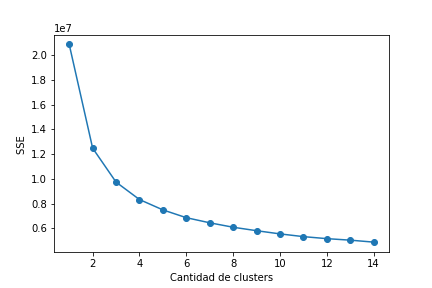
\includegraphics[width = 2in]{img/kmeans/elbow-join.png}
        \caption{Método elbow}
    \end{subfigure}
    \begin{subfigure}{.4\textwidth}
        \centering
        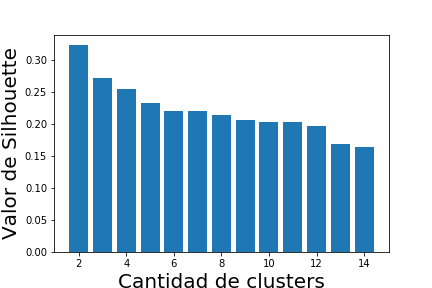
\includegraphics[width = 2in]{img/kmeans/silhouette-join.png}
        \caption{Silhouette score}
    \end{subfigure}
    \caption{Cantidad de clusters óptima}
    \label{fig:elbow-silhouette-join}
\end{figure}

En este caso se puede ver como la caída de la curva en el método elbow es mucho mas suave y no tan marcada como en el primer caso. Si bien parece que de nuevo 3 clusters sería el número ideal, también 4 o 5 obtuvieron buenos valores de silhouette. Vamos a elegir el número en 3 para poder compararlo con las experimentaciones previas y 4 para ver como se comporta contra el mismo conjunto de datos pero con la elección previa de 3 grupos. Siendo esta última unión la que mejores índices tiene y un valor muy superior cuando se eligen 4 grupos.

\begin{table}[H]
    \centering
    \begin{tabular}{|c|c|}
        \hline
        Conjunto de datos & Indice de Rand \\
        \hline
        Solo atributos alto nivel & 0.122 \\
        Solo atributos de bajo nivel & 0.151 \\
        Unión con 3 clusters & 0.186 \\
        Unión con 4 clusters & 0.245 \\
        \hline
    \end{tabular}
    \caption{Rand index}
    \label{tab:rand-kmeans-af-3-aa-3-join-3-join-4}
\end{table}

A continuación se puede apreciar como fueron ubicados las canciones en los diferentes grupos, primero con un número de clusters de 3 y luego de 4

\begin{table}[H]
    \centering
    \begin{tabular}{|c|c|c|c|}
        \hline
        & \multicolumn{3}{ c| }{Clusters} \\
        \hline
        Género & 0 & 1 & 2 \\
        \hline
        ambient & 219 & 22 & 219 \\
    	classical & 273 & 30 & 102 \\
    	drum-and-bass & 17 & 434 & 0 \\
    	jazz & 287 & 80 & 59 \\
    	world-music & 277 & 118 & 68 \\
        \hline
    \end{tabular}
    \caption{Géneros musicales en 3 grupos}
    \label{tab:cross-kmeans-join-3}
\end{table}

\begin{table}[H]
    \centering
    \begin{tabular}{|c|c|c|c|c|}
        \hline
        & \multicolumn{4}{ c| }{Clusters} \\
        \hline
        Género & 0 & 1 & 2 & 4 \\
        \hline
        ambient & 83 & 203 & 17 & 157 \\
		classical & 252 & 101 & 5 & 47 \\
		drum-and-bass & 8 & 0 & 427 & 16 \\
		jazz & 132 & 44 & 65 & 185 \\
		world-music & 77 & 52 & 98 & 236 \\
        \hline
    \end{tabular}
    \caption{Géneros musicales en 4 grupos}
    \label{tab:cross-kmeans-join-4}
\end{table}

De nuevo \textbf{drum-and-bass} al igual que en los previos experimentos resultó ser siempre el estilo más concentrado. Particularmente con la elección de 4 grupos se puede apreciar otras relaciones interesantes entre los estilo restantes. Por ejemplo en el cluster 0 hay muchos pistas del género \textit{classic} y \textit{jazz}, en el grupo 1 gran cantidad de \textit{ambient} y en último el número 3 se observa gran concentración de canciones del género \textit{classic} \textit{world-music}, \textit{jazz} y \textit{ambient}.

\begin{figure}[H]
    \begin{subfigure}{.4\textwidth}
        \centering
        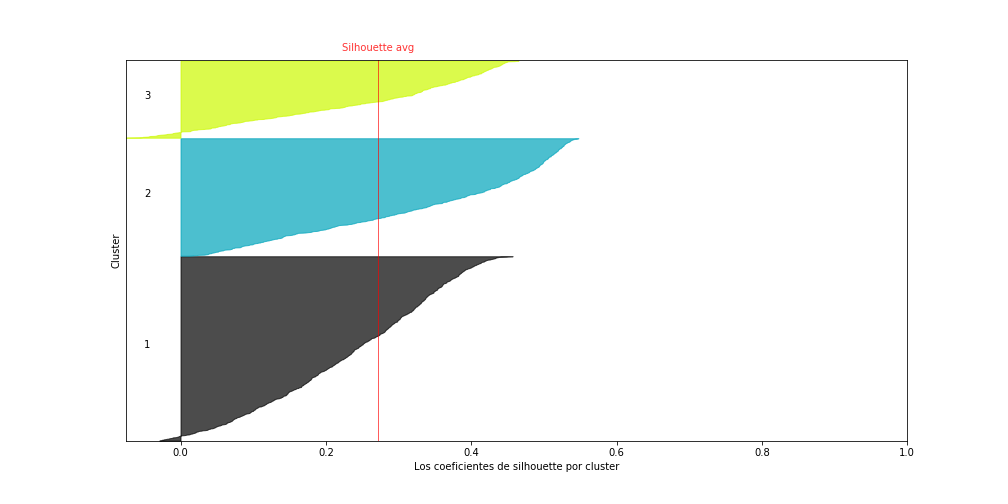
\includegraphics[width = 2in]{img/kmeans/silhouette-join-3-eo.png}
        \caption{Silhouette para 3 clusters}
    \end{subfigure}
    \begin{subfigure}{.4\textwidth}
        \centering
        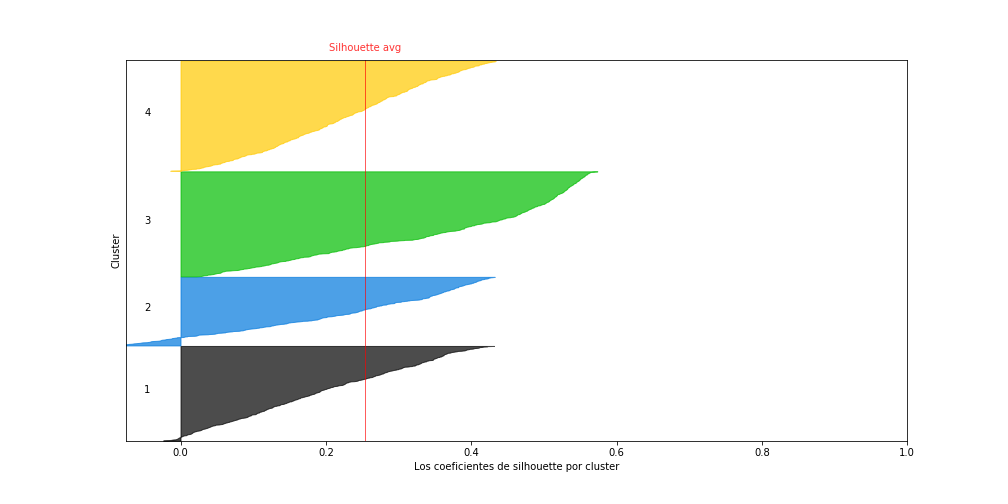
\includegraphics[width = 2in]{img/kmeans/silhouette-join-4-eo.png}
        \caption{Silhouette para 4 clusters}
    \end{subfigure}
    \caption{Silhouette en la unión de los atributos}
    \label{fig:silhouette-join-3-4}
\end{figure}

La elección de 4 clusters en este caso parece mucho más interesante ya que se comienzan a descubrir mejores relaciones y similitudes entre las canciones gracias a la unión de los datos.

Como se verá más adelante los valores obtenidos para éstas mismas métricas fueron superiores ya que se trata de métodos más complejos y que en general funcionan mejor. Es por eso que en este caso no se van a realizar más experimentos ni analizar métricas.

El algoritmo \textbf{KMeans} si bien no es el mejor y la implementación de \textit{Scikit Learn} no ofrece mucha parametría con la cuál experimentar, es muy útil para comenzar con cualquier tipo de análisis ya que es un método muy rápido que no requiere ningún tipo de supervisión y sirve como métrica con la cuál comparar al resto de los algoritmos.



\newpage
\section{Experiencia Jerarquico}
%!TEX TS-program = xelatex
%!TEX encoding = UTF-8 Unicode
Se utilizó el algoritmo \textbf{AgglomerativeClustering} de la librería sklearn extra.cluster y con la métrica de distancia euclidean.

\subsection{Resultados}
\subsubsection{Audio Features}
\begin{center}\textbf{Dendogramas}\end{center}


En un primer analisis, tuvimos que decidir que tipo de distancia utilizariamos para formar los clusters, la funcion AgglomerativeClustering nos daba cuatro opciones de linkage criterion:

\begin{itemize}
  \item \textbf{ward} Minimiza la varianza de los clusters que son mergeados.
  \item \textbf{average} Computa la distancia media de cada observacion de dos conjuntos.
  \item \textbf{single} Usa la maxima distancia entre todas las observaciones de dos conjuntos.
  \item\textbf{complete} Usa la maxima distancia entre todas las observaciones de dos conjuntos.
\end{itemize}

Se generan los 4 dendogramas para estudiar que criterio agrupa mejor los datos.

\begin{figure}[H]
{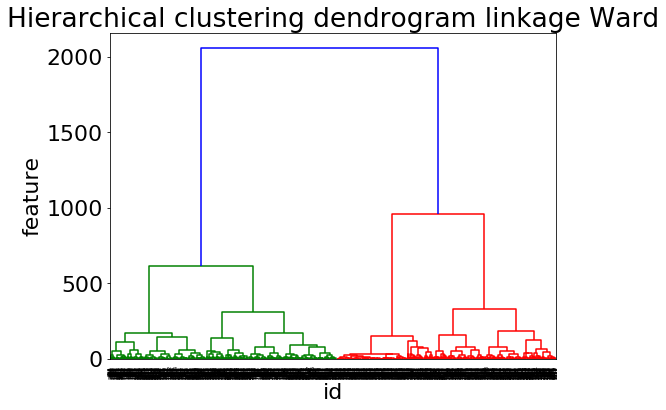
\includegraphics[width = 3in]{img/imagenes/jerarquico_AF/dendongrama_ward.png}} 
{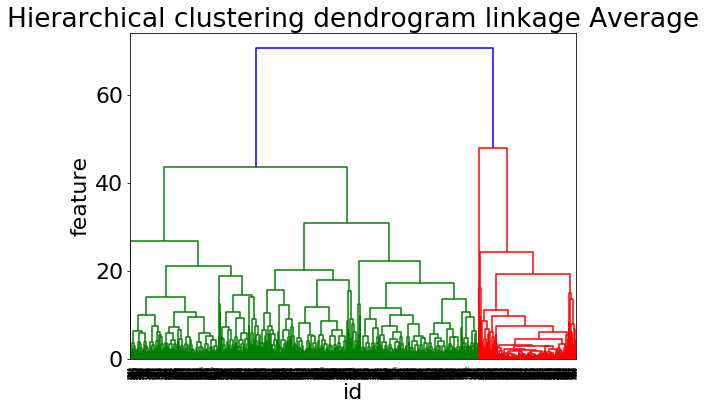
\includegraphics[width = 3in]{img/imagenes/jerarquico_AF/dendongrama_average.png}}\\
{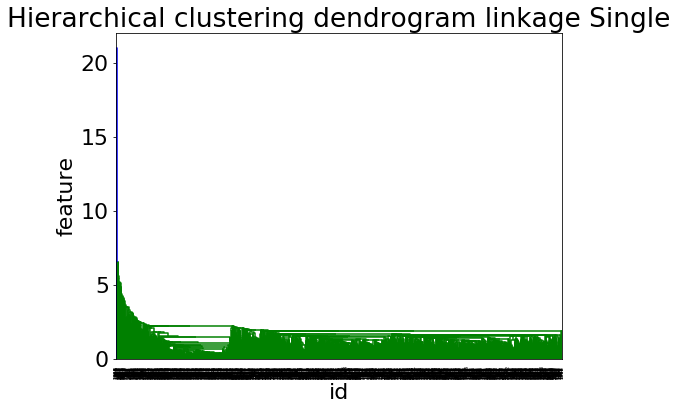
\includegraphics[width = 3in]{img/imagenes/jerarquico_AF/dendongrama_single.png}}
{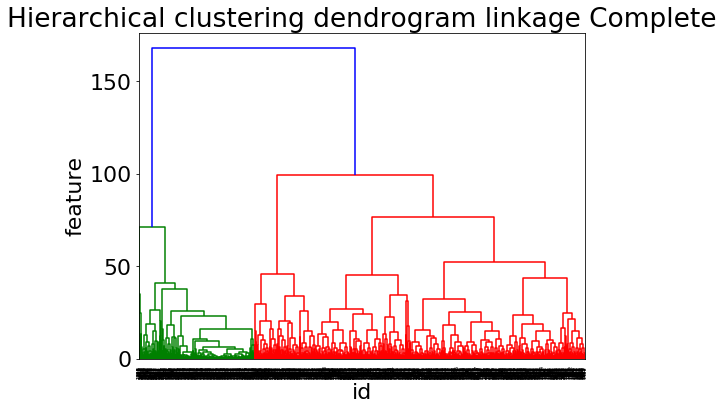
\includegraphics[width = 3in]{img/imagenes/jerarquico_AF/dendongrama_complete.png}} 
\label{Comparativa entre linkage criterions}
\end{figure}

Al revisar la salida de los distintos linkages, lo que podemos observar es que el metodo \textbf{ward} es quien esta manteniendo un mayor balance entre los distintos clusters. Revisando en detalle dicho dendograma, podemos concluir en principio que una separacion natural podria ser en 2, 3 o 4 clusters ya que determinamos que con esta cantidad se podria generar un balanceo entre el tamaño de los mismos.

\begin{figure}[H]
    \centering
    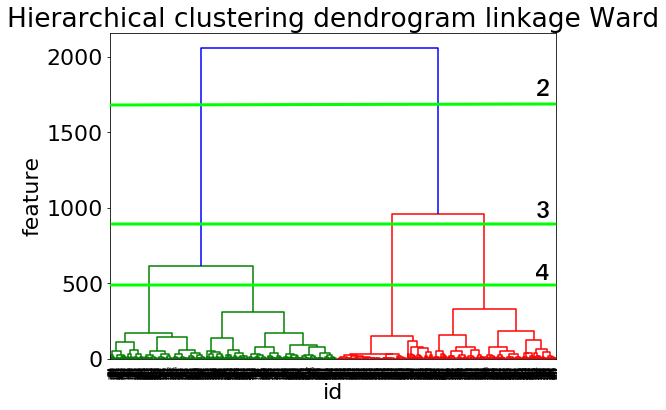
\includegraphics[width=\textwidth]{img/imagenes/jerarquico_AF/dendongrama_ward_clusters.png}
    \caption{Posibles separaciones en Clusters}
    \label{fig:clusters}
\end{figure}

Si bien dicha apreciación podria ser verdadera, nos disponemos a estudiar distintos coeficientes y tecnicas que nos permitiran entender cual es el mejor \textbf{K} para este metodo.

\begin{center} \textbf{Coeficiente de Silhouette} \end{center}
Para determinar en que cantidad de clusters conviene mas realizar la separaciones, nos basamos en el coeficiente de Silhouette, el cual nos da una medida para saber cual es el \textbf{K} óptimo para construir la separación. Se realizó el computo de dicho coeficiente para 2, 3, 4, 5 y 6 divisiones como para tener una imagen mas completa sobre como se estan comportando los datos.

\begin{figure}[H]
    \centering
    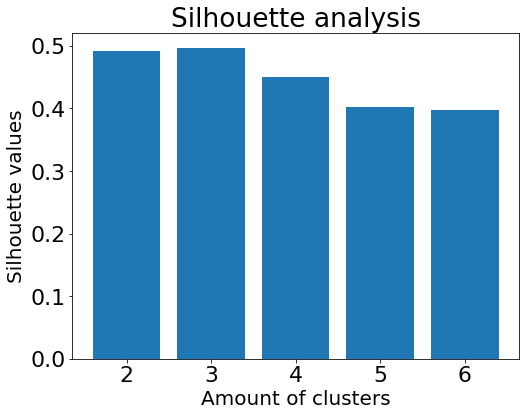
\includegraphics[width=\textwidth]{img/imagenes/jerarquico_AF/silhouette_general.png}
    \label{fig:silGeneral}
\end{figure}

\newpage
Como podemos ver en el resultado, claramente con un \textbf{K=2} o \textbf{K=3} se obtiene el mejor coeficiente, nos disponemos ahora a realizar un analisis un poco mas profundo sobre estos valores para tomar una decision, graficaremos los coeficientes comparando ahora para 2, 3 divisiones. 

\begin{figure}[h]
{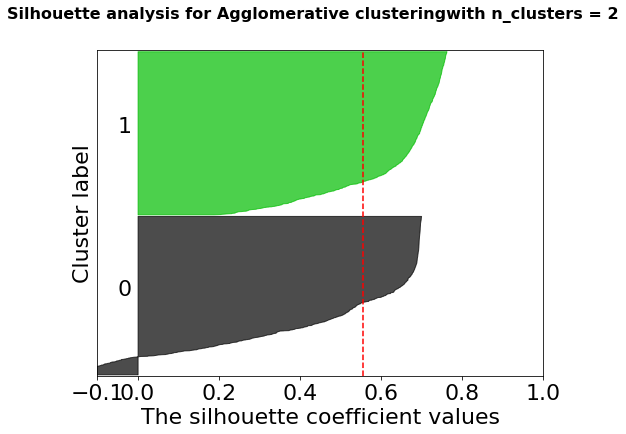
\includegraphics[width = 3in]{img/imagenes/jerarquico_AF/silhouette_2.png}} 
{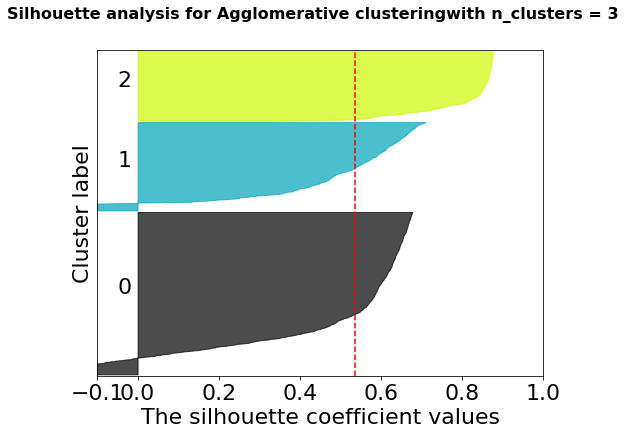
\includegraphics[width = 3in]{img/imagenes/jerarquico_AF/silhouette_3.png}}\\
\label{fig: Comparativa entre Silhouette}
\end{figure}

\begin{table}[H]
    \centering
    \begin{tabular}{|c|c|}
		\hline
        Cantidad de clusters & Silhouette Score \\
        \hline
        2 & 0.5566\\
        3 & 0.5362\\
        \hline
    \end{tabular}
    \caption{Silhouette Score}
    \label{tab:clus-sil}
\end{table}

Si bien se obtiene un mejor coeficiente para un \textbf{K=2}, como la diferencia entre este y el \textbf{K=3} es muy pequeña seleccionaremos al K=3 ya que nos permite contar con mas agrupaciones y poder lograr una separacion en clusters mas interesante.

\begin{center} \textbf{Cross table} \end{center}
Para entender a mas a detalle que tan bien se realizo la clasificaciones se genera la siguiene tabla donde se aprecia el agrupamiento de generos en los dinstios clusters.

\begin{table}[H]
    \centering
    \begin{tabular}{|c|c|c|c|}
        \hline
        & \multicolumn{3}{ c| }{Clusters} \\
        \hline
        Género & 0 & 1 & 2 \\
        \hline
        ambient & 274 & 154 & 32 \\
        classical & 308 & 72 & 25 \\
        drum-and-bass & 42 & 55 & \textbf{354} \\
        jazz & 240 & 153 & 34 \\
        world-music & 255 & 175 & 33 \\   
        \hline
    \end{tabular}
    \caption{Géneros musicales y grupos}
    \label{tab:cross-af}
\end{table}

Podemos observar que el mejor agrupamiento lo tenemos en el cluster 2, con el genero \textbf{drum-and-bass}. Al igual que  con K-means y con PAM dicho genero es quien concentro en un cluster la mayor cantidad de observaciones.
Se dispone a analizarlos índices de RAND y VanDongen para evaluar si los agrupamientos son similares para los distintos conjuntos de datos.

\begin{table}[H]
	\centering
	\begin{tabular}{ |c|c|c| }
		\hline 		
 		Cantidad de clusters & Indice RAND & Indice VanDongen\\ 
 		\hline
 		2 & 0.1918 & 0.7805\\ 
 		3 & 0.3085 & 0.7575\\
 		\hline    
	\end{tabular}
     \label{tab:clus-rand-vand}
\end{table}

Si bien tomamos la decisión de elegi un \textbf{K=3}, algunos analisis los haremos con \textbf{K=2} tambien para comparar en todo momento que nuestra
elección haya sido adecuada.

Con el índice de VanDongen se observa un alto grado de pureza con los clusters analizados, mas de un $75\%$.
Para el índice RAND podemos comentar que el porcentaje de decisiones correctas del cluster es de
$30\%$ sin embargo es de esperable tener un porcentaje bajo ya que se están realizando agrupaciones de 3
clusters a diferencia de las 5 etiquetas de género en los datos.

\begin{center} \textbf{Componentes principales} \end{center}
A continuación se realizó análisis de componentes principales con la finalidad de reducir la dimensionalidad del data set estudiado y
asi poder lograr una representación gráfica de la division en 3 clusters.

\begin{figure}[H]
    \centering
    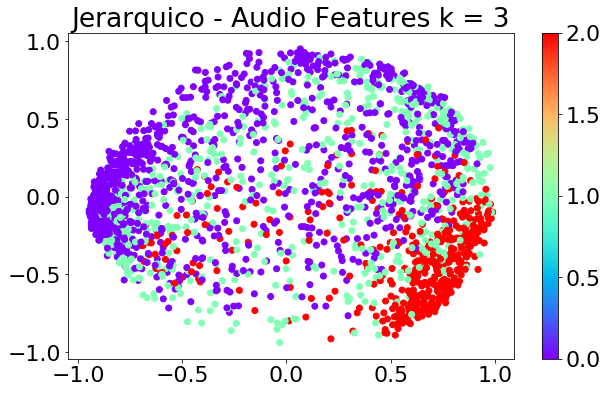
\includegraphics[width=\textwidth]{img/imagenes/jerarquico_AF/pca_3clusters.png}
    \caption{PCA}
    \label{fig:pca}
\end{figure}

Dadas las componentes 1 y 2 se observa un buen conglomerado diferenciado en especial para el cluster 2, drum-and-bass, el cual presenta su mayor densidad
en la parte positiva de la primer componente y negativa de la segunda. Lo sigue en densidad el cluster 0, y por ultimo el cluster 1 el cual presenta valores mas distribuidos y casi sin compactarse.
Cabe destactar que en el centro del grafico, proximo al valor (0,0) se pueden encontrar elementos de los 3 clusters.



\subsubsection{Audio Analisis}
Comenzamos realizando una analisis de Silhouette sobre los distintos tipos de data set $timbres\_avg$, $timbres\_std\_dev$, $pitches\_avg$ y $pitches\_std\_dev$
Para hacer esto, nos basamos en la experiencia obtenida con Audio Features, y utilizamos la misma medida Ward y la misma cantidad de clusters optimos encontrada hasta el momento de 3.

\begin{figure}[H]
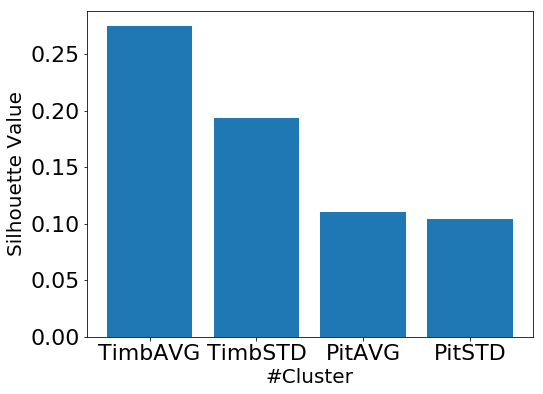
\includegraphics[width=\textwidth]{img/imagenes/jerarquico_AA/silhouette_avgstd.png}
\end{figure}
\begin{center}Comparativa general\end{center}

\begin{table}[H]
	\centering
	\begin{tabular}{ |c|c|c| }
		\hline
 		Data Set & Cantidad de clusters & Indice RAND\\
 		\hline
 		timbres avg & 3 & 0.1690\\
        timbres std & 3 & 0.0666\\
        pitches avg & 3 & 0.0754\\
        pirches std & 3 & 0.0231\\
        \hline
	\end{tabular}
     \label{tab:rand-ds}
\end{table}

Observando los valores de Silhouette, la mejor manera de clasificar a las canciones para este dataset es a traves de la media de \textbf{timbres average}.
Como proximo paso, se procede a realizar una junta entre el dataset de $audio\_features$ con $audio\_analysis$ que ya contenia el promedio de los timbres.
Para realizar un analisis mas profundo sobre este nuevo data set.

\begin{figure}[H]
    \centering
    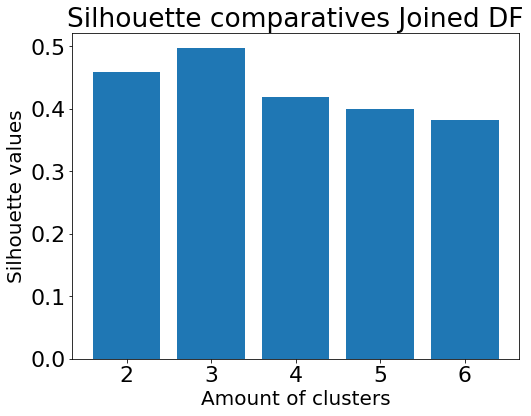
\includegraphics[width=\textwidth]{img/imagenes/jerarquico_AA/silhouette_joinedDF.png}
    \caption{Silhouette Joined DF}
    \label{fig:silJoinedDF}
\end{figure}

\begin{table}[H]
    \centering
    \begin{tabular}{|c|c|}
    	\hline
        Cantidad de clusters & Silhouette Score \\
        \hline
        2 & 0.4582\\
        3 & 0.4968\\
        4 & 0.4192\\
        5 & 0.3997\\
        6 & 0.3822\\
        \hline
    \end{tabular}
    \caption{Sil full data set}
    \label{tab:sil-fullds}
\end{table}

Nuevamente hacemos un balance entre el valor que nos arroja el Silhouette y la mejor configuracion de cantidad de K. Al igual que antes, tanto para \textbf{K=2}, \textbf{K=3}, \textbf{K=4} los valores son muy similares decidimos ir por \textbf{K=3} ya que tiene el valor mayor y ademas poder tener cierto grado de comparacion con el trabajor realizado antes.
Nos proponemos ahora a calcular los indices RAND y VanDongen

\begin{table}[H]
	\centering
	\begin{tabular}{ |c|c|c| }
		\hline
 		Cantidad de clusters & Indice RAND & Indice VanDongen\\
 		\hline
		 2 & 0.1855 & 0.6502\\
         3 & 0.3160 & 0.5194\\
         \hline
	\end{tabular}
     \label{tab:rand-ds}
\end{table}

El índice de VanDongen da un grado de pureza medio, aproximadamente un $51\%$ para el \textbf{K=3},
para el indice RAND podemos afirmar que el porcentaje de decisiones correctas del cluster es de un $31\%$, muy similar al anterior
analisis y esperable ya que estamos teniendo 3 clusters vs las 5 etiquetas que hay.

\begin{center} \textbf{Cross table} \end{center}
Para entender a mas a detalle que tan bien se realizo la clasificaciones se genera la siguiene tabla donde se aprecia el agrupamiento de generos en los dinstios clusters.

\begin{table}[H]
    \centering
    \begin{tabular}{|c|c|c|c|}
        \hline
        & \multicolumn{3}{ c| }{Clusters} \\
        \hline
        Género & 0 & 1 & 2 \\
        \hline
        ambient & 334 & 24 & 102 \\
        classical & 386 & 17 & 2 \\
        drum-and-bass & 0 & 22 & \textbf{429} \\
        jazz & 158 & 232 & 36 \\
        world-music & 93 & 334 & 36 \\  
        \hline
    \end{tabular}
    \caption{Géneros musicales y grupos full df}
    \label{tab:cross-fulldf}
\end{table}

Al revisar la conformacion de los clusters, nuevamente podemos apreciar que el genero \textbf{drum-and-bass} es quien se concentra en su mayoria
en el cluster 3.

\begin{center} \textbf{Componentes principales} \end{center}
Nuevamente realizamos un análisis de componentes principales con la finalidad de reducir la dimensionalidad del data set estudiado y asi poder lograr una representación gráfica de la division en 3 clusters.

\begin{figure}[H]
    \centering
    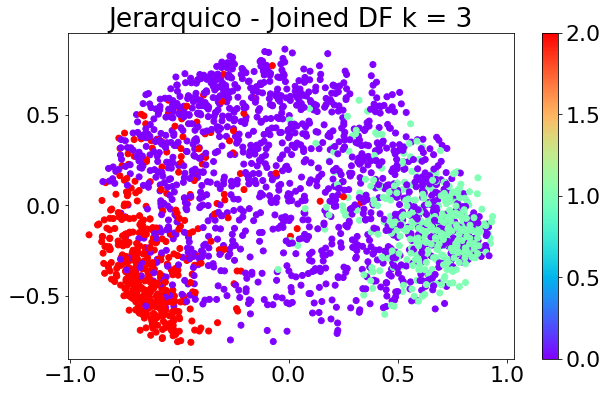
\includegraphics[width=\textwidth]{img/imagenes/jerarquico_AA/pca_joinedDF_3clusters.png}
    \caption{PCA Joined DF}
    \label{fig:pcaJoinedDF}
\end{figure}

Dadas las componentes 1 y 2 se observa un buen conglomerado diferenciado en especial para el cluster 2, drum-and-bass, el cual tiene su mayor cantidad de valores en la zona de proyeccion negativa de la primer y segunda componente. Un caso algo diferente es el del cluster 1 que si bien logra algo de aglomeración, se proyecta casi en su totalidad en la parte positiva de la primer componente e intercalando entre positivo y negativo para la segunda componente. Por ultimo esta el cluster 0, el cual muestra mayor esparcimiento y ocupando valores positivos y negativos de ambas componentes.
Se aprecia por ultimo, una separacion mas marcada entre el cluster 1 y 2, mientras que el 0 esta mas desparramado.



\newpage
\section{Experiencia algoritmo PAM}
Se utilizó el algoritmo \textbf{KMedoids} de la librería sklearn extra.cluster y con la métrica de distancia euclidean.
\subsection{Métodos}
Con el dataset de audio features ejecutamos el algoritmo para distintos k midiendo en cada uno de ellos el promedio del coeficiente de Silhouette para así determinar el k óptimo a utilizar en el análisis.

Los k utilizados fueron [2, 3, 4, 5, 6, 8, 10] y resultados obtenidos los siguientes:

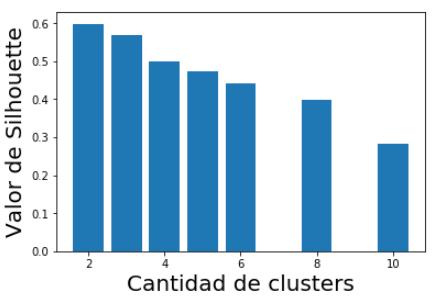
\includegraphics[width=\textwidth]{img/imagenes/2PAM_silohuete_k}
\begin{center} Gráfico valores de silhouette \end{center}

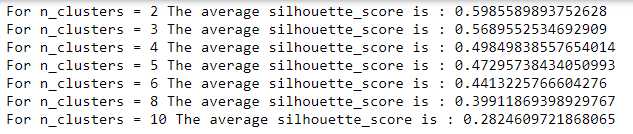
\includegraphics[width=\textwidth]{img/imagenes/1PAM_silohuete}
\begin{center}Coeficiente de Silhouette para varias ejecuciones.\end{center}

Con el coeficiente de Silhouette decidimos continuar con el k=3 debido a que presentaba un coeficiente cercano al n=2 y así podríamos observar más cantidad de agrupaciones, de igual manera se realizó gráfico para k=2 y k=3 para dejar evidencia de los parecido de los algoritmos con ambos k.

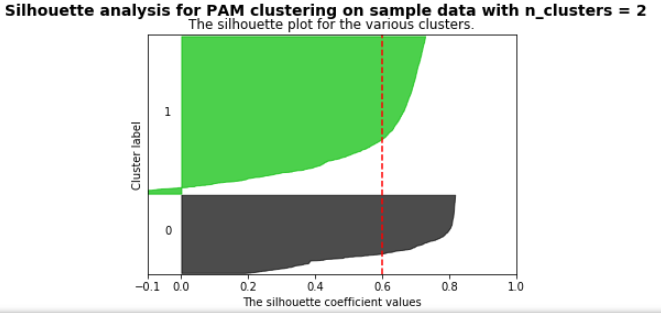
\includegraphics[width=\textwidth]{img/imagenes/3PAM_silohuete_k2}

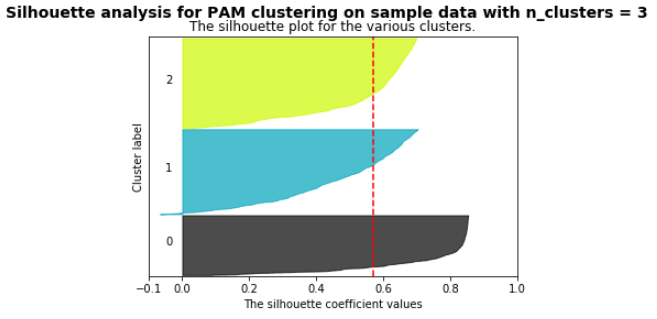
\includegraphics[width=\textwidth]{img/imagenes/4PAM_silohuete_k3}


Importante acotar que para las ejecuciones se utilizaron las variables con sus escalas originales, no se aplica normalización ni estandarización.

Con k=3 logramos un coeficiente de 0.5689 lo cual es un número bastante aceptable a nivel general.  Para conocer el nivel de concentración de cada cluster obtenemos el cálculo agrupado.

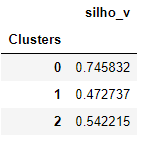
\includegraphics[width=7cm, height=6cm]{img/imagenes/6silohu_group}

Silhouette por cluster.

Se observa que el cluster "0" posee un coeficiente más alto que el resto con lo cual la observaciones pertenecientes a se encuentran mejor agrupadas. Para ver que tan bien clasificó nuestro clustering con respecto a los géneros de música que se tenían en el dataset realizamos una crosstable.

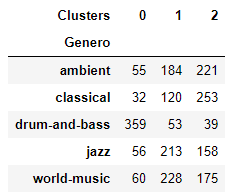
\includegraphics[width=7cm, height=6cm]{img/imagenes/5crosstab_PAM}

Se valida que el género mejor agrupado es \textbf{drum-and-bass} el cual presenta gran concentración en el cluster 0. Esta buena agrupación para este género coincide con los resultados observados en el análisis realizado con el método de clustering K-Means.

Utilizamos los índices de RAND y VanDongen para evaluar si los agrupamientos son similares para los distintos conjuntos de datos.

Con el algoritmo de KMedoids y la configuración antes indicada se obtuvieron los siguientes valores.

Índice Rand para Algoritmo PAM con 3 clusters: 0.1240

Índice VanDongen para Algoritmo PAM con 3 clusters: 0.7405

Con el índice de VanDongen se observa un alto grado de pureza con los clusters analizados.

Para el índice RAND podemos comentar que el porcentaje de decisiones correctas del cluster es de 12\% sin embargo es de esperable tener un porcentaje bajo ya que se están realizando agrupaciones de 3 clusters a diferencia de las 5 etiquetas de género en los datos.

A continuación se realizó Análisis de Componentes con la finalidad de reducir la dimensionalidad de nuestro dataset para poder realizar una representación gráfica de nuestros clusters.

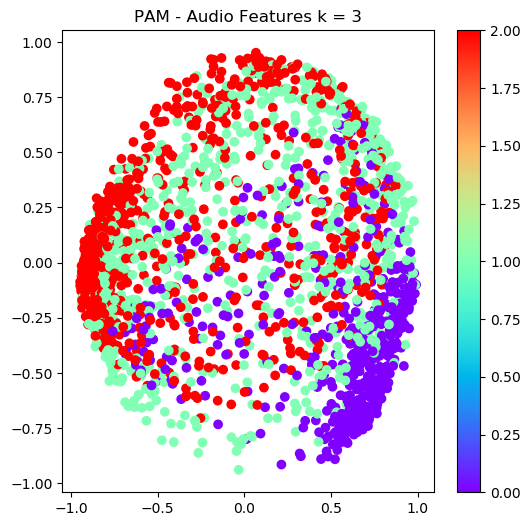
\includegraphics[width=10cm, height=10cm]{img/imagenes/7PAM_pcaV2}

Con las componentes 1 y 2 se observa un buen conglomerado diferenciado en los cluster 2 y 0, sin embargo el cluster 1 se encuentra más distribuido a lo largo y ancho del gráfico. Podemos decir que el cluster "0" drum-and-bass se caracteriza en su mayoría por tener valores positivos en la primera componente (eje x) y negativos en la segunda componente (eje y), mientras que el cluster 2 presenta en su mayoría negativos en x y positivos cercanos a cero en la segunda componente.    

También podemos ver una separación un poco más clara entre el cluster 0 y 1 que el cluster 2 con respecto al resto.

\newpage
\section{Experiencia Algoritmo DBSCAN}
Como acercamiento y validación de otros métodos de clustering decidimos probar con el algoritmo DBSCAN el cual al estar basado en densidad permite agrupar de mejor manera datos que no posean una forma particular.

Con una configuración de eps = 2 un min sample= 25 y métrica euclidean se obtuvieron 3 clusters los cuales presentaban una métrica de silhouette de 0.1564 y la siguiente crossTable:

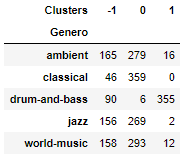
\includegraphics[width=7cm, height=6cm]{img/imagenes/8DBSCAN_ct.PNG}

Vemos una muy buena clasificación para el género drum-and-bass en el cluster 1, sin embargo el resto de los géneros se encuentran muy distribuidos por el resto de los cluster lo cual puede ser el motivo de obtener un coeficiente de silhouette tan bajo.

En el siguiente gráfico podemos observar las clasificación del algoritmo en baja dimensionalidad (Utilizamos PCA para reducir las dimensiones).

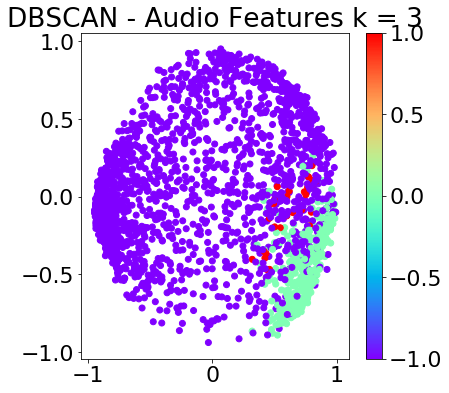
\includegraphics[width=12cm, height=10cm]{img/imagenes/9DBSCAN_pca}

Tal como se comentó anteriormente la clasificación del género drum-and-bass se encuentra concentrada en el cluster 1 y lo podemos observar en el gráfico de las componentes principales.

Podemos comentar que las causas de la baja performance de este algoritmo se debe a que precisamente se trata de un método basado en densidad y según lo observado durante la elaboración del pre TP1 en la sección de scatter plot´s muchos de los features del dataset presentaban altas concentraciones y se mezclaban los distintos géneros musicales.

\newpage
\section{Clustering de secciones dentro de una pista}
Para este análisis se seleccionó una pista de Timbres de los datos de Audio Analysis, específicamente la pista cuyo id es "00At7PWydsvg7g5xgaYan9", es una canción de genero Electro/Pop: All I Know - Matrix \& Futurebound ft. Luke Bingham.

Se realizó una matriz de recurrencia con los datos normalizados y la serie temporal de la pista interpolada obteniendo los siguientes resultados:

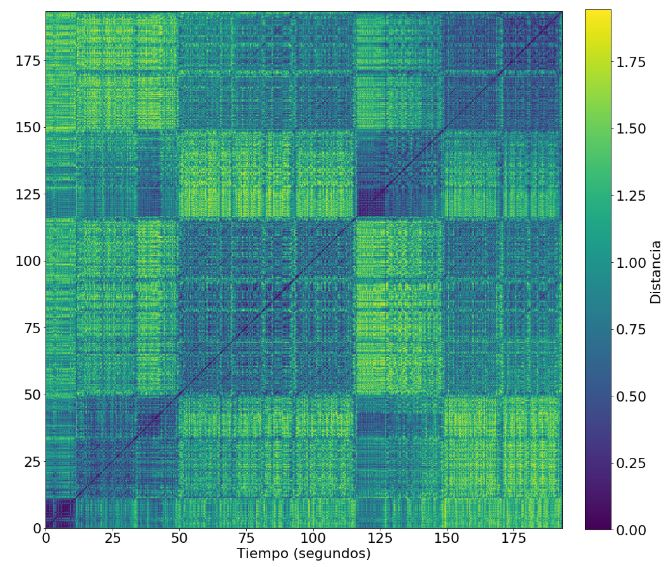
\includegraphics[width=12cm, height=10cm]{img/imagenes/10_matriz_recurrencia}

Lo primero que se puede destacar es en los primeros segundos de la canción, se ve claramente una intro que es bastante distinta al resto, seguida de un par de secciones parecidas entre sí (estribillos y coros). Se puede observar también en el segundo 125 un segmento de la canción con características similares al intro.

Para validar los resultados del análisis se escuchó la pista validando que la intro se caracteriza por un sonido más instrumental/electrónico, sin vocalización, similar al del segundo 125. El resto de la canción tiene vocalizaciones con tonos muy uniformes. 

Así mismo, para corroborar este análisis se utilizó el algoritmo de clustering de KMeans para identificar distintos grupos dentro de la pista, obteniéndose los siguientes resultados medidos con la métrica de Silhouette:

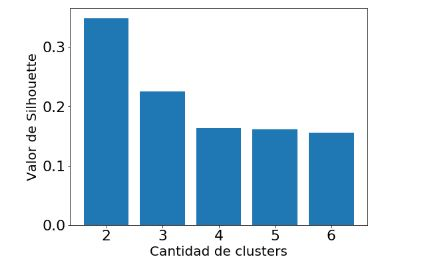
\includegraphics[width=12cm, height=10cm]{img/imagenes/11cantidad_clusters}

Los resultados obtenidos indican una clara identificación de dos clusters, que según lo escuchado en la pista y lo visto en la matriz de recurrencia serían las secciones instrumentales/electrónicas y las secciones donde hay vocalización. Si bien la mejor distinción es la de k=2, con k=3 también se observa una leve mejora con respecto a los k > 3, esto puede ser a la diferenciación de la vocalización escuchada en los estribillos y el coro.

\newpage
\section{Conclusiones}
%!TEX TS-program = xelatex
%!TEX encoding = UTF-8 Unicode

\begin{itemize} 

\item El análisis de cluster permite no solo el agrupamiento de datos para su estudio, sino una manera simple de conocer como es la morfología de los datos, encontrar relaciones y ser un puntapié para empezar a conocer de que se trata un data set. Por medio de dinstintas técnicas de clustering en este trabajo pudimos probar y experimentar sobre como algunos conceptos que en principio parecen simples, como ser en cuantos cluster queremos que cierto algoritmo separe nuestros datos, se vuelven muy complejos al momento de comenzar la exploración ya que uno fácilmente se puede verse tentado a ultiliar algún dato del dominio. En este trabajo, los géneros parecían una partición natural y en cierto modo fue nuestra primer opción, luego cuando íbamos iterando por las distintas técnicas y cálculos nos fuimos dando cuenta que grupos de datos que por su etiqueta parecían dar origen a un agrupamiento en particular no eran mas que partes de un agrupamiento mas general. 

\item Es fundamental contar con técnicas no solo numéricas sino gráficas para el análisis de los distintos coeficientes y resultados, en muchos casos puede haber pequeñas diferencias numéricas pero que llevadas a gráficos hacen que su diferencia hagan tomar una decisión u otra. En este trabajo, la manera de graficar los coeficientes de Silhouette nos fue de gran utilidad para elegir entre uno u otro K para partir nuestro conjunto de datos. 

\item El análisis por PCA nos permitió poder graficar los clusters y así poder entender como se estaban agrupando los datos en ciertos clusters y como se formaban regiones densas y regiones mas claras, también aprovechamos para ver como algunas zonas contaban con datos de mas de un cluster y otras zonas tenían datos exclusivos. De alguna forma nos sirvió para bajar a tierra los números o los datos duros de las tablas, permitiéndonos en una mirada rápida tener una idea de como estaban formados los clusters, que densidades tenían y que tan desparramados estaban sus datos. 

\item La manera de calcular la distancia entre los puntos o conjuntos de puntos de los cluster resulta fundamental para poder realizar un clustering adecuado, como vimos en Jerárquicos la diferencia entre la separación que formaba Ward y Simple era muy evidente. En un primer momento, pensamos que la distancia promedio seria la mejor, ya que como no teníamos conocimiento previo del dominio o de que forma se podrían formar estos clusters nos aventuramos al pensar que el promedio era quien mejor podría representarlos. Nuestra sorpresa vino al conocer que solo Ward era la métrica que nos estaba arrojando una resultado que nos convencía. 

\item En los tres métodos donde pudimos estudiar la configuración de los clusters, vimos que el genero drum-and-bas fue quien se acumulo mayoritariamente en uncluster diferenciándose del resto de los géneros. 

\item Como en todos los casos donde se tenga que trabajar con datos de un cierto dominio, siempre contar con información del mismo es una ventaja, ya que permite pensar pre conceptos que luego uno puede desafiar con los datos duros y poder re preguntarse mas de una vez si un resultado es el correcto. Ponemos nuevamente el ejemplo de los géneros, donde mas de una vez forzamos los cálculos para volver a comprobar si una separación en géneros no era la correcta o la esperada.

 \end{itemize}

\printbibliography

\end{document}

